\chapter{Équations aux différences}
    \section{Introduction}
        Les équations aux différences sont au cœur de la modélisation de nombreux phénomènes dynamiques, lorsque leur formulation s'exprime en temps discret.

        L’étude des équations aux différences trouve ses racines dans les travaux des mathématiciens du XVIIe siècle, comme Pierre de Fermat et Blaise Pascal, qui utilisaient des suites arithmétiques et géométriques pour comprendre des phénomènes de croissance. Par exemple, les fameux nombres de Fibonacci, introduits en Occident par Leonardo Fibonacci au XIIIe siècle pour modéliser la croissance d’une population de lapins, sont représentés par une équation aux différences simple, mais élégante.

        Ce chapitre vise à fournir les outils nécessaires pour comprendre, formuler et résoudre des équations aux différences, en particulier celles de premier ordre et celles linéaires d'ordre supérieur. Nous allons aborder les notions fondamentales, de la définition et de la forme générale d'une équation aux différences, jusqu’à la solution de systèmes linéaires et la compréhension des phénomènes de stabilité et de convergence des solutions.
        
        Nous commencerons par explorer les notions fondamentales des équations aux différences d’ordre supérieur. Puis, nous présenterons des théorèmes sur l'existence et l'unicité des solutions, ainsi que des méthodes de résolution pour les équations linéaires homogènes et non homogènes. Les concepts de solution particulière, solution homogène, et solution générale seront abordés en détails. La fin du chapitre sera dédiée à l’étude de la stabilité des solutions et aux techniques de résolution des équations aux différences à coefficients constants. \robin{A confirmer, mais normalement ces notions ont déjà été vues en math discrètes.}
        
    \section{Rappels théoriques}
        \subsection{Équations aux différences}
            \begin{definition}{Équation aux différences} 
                Soit $x_k = x(k) \in X$ l’état scalaire d’un système dynamique à l’instant $k \in \mathbb{N}$ et $f: \mathbb{N} \times X^n \to X$ une fonction donnée. Une équation aux différences d'ordre $n$ décrit l'évolution d'un système dynamique en exprimant l'état futur $x(k+n)$ en fonction des états précédents $x(k+n-1), \dots, x(k)$. Cette relation récursive s'écrit:
                \begin{equation}\label{eq:eq_difference}
                    x(k+n) = f(k, x(k+n-1), \dots, x(k))
                \end{equation}
                où $f$ est connue. Ce type d'équation est appelé \textit{équation aux différences d’ordre $n$ en forme normale}.
            \end{definition}
    
            \begin{theorem}{Existence et unicité de la solution}
                Pour une équation aux différences d'ordre $n$, il existe une unique solution dès lors que $n$ valeurs initiales sont fixées. Aucune hypothèse supplémentaire n'est requise sur la forme de la fonction $f$ pour garantir cette unicité.
            \end{theorem}
            L'unicité de la solution est essentielle, car elle assure que pour une condition initiale donnée, le comportement du système est entièrement déterminé.

        \subsection{Équation aux différences linéaire}
            Dans ce chapitre, nous nous concentrons sur le cas spécifique des équations aux différences linéaires.
            \begin{definition}{Équation aux différences linéaire}
                Une équation aux différences est dite \textit{linéaire d’ordre $n$} si elle peut être exprimée sous la forme:
                \begin{equation}\label{eq:eq_difference_lineaire}
                    a_n(k)x(k+n)+a_{n-1}(k)x(k+n-1)+\cdots+a_0(k)x(k) = g(k)
                \end{equation}
                où $a_i(k)$ et $g(k)$ sont des fonctions données pour $i = 0, \dots, n$. Ici, $a_i(k)$ représente les coefficients de l'équation et $g(k)$ est un terme extérieur.
            \end{definition}
        
            Si les coefficients $a_i(k)$ sont constants, l'équation est dite \textit{invariante} (ou \textit{stationnaire}). Typiquement, le comportement ne varie pas en fonction de paramètres comme le temps ou la position. On distingue aussi la notion d'équation homogène:
            \begin{definition}{Équation aux différences linéaire homogène}
               Si $g(k) = 0$ pour tout $k$, l'équation \ref{eq:eq_difference_lineaire} devient:
                \begin{equation}
                    a_n(k)x(k+n)+a_{n-1}(k)x(k+n-1)+\cdots+a_0(k)x(k) = 0
                \end{equation}
                et est dite \textit{homogène}.
            \end{definition}

            Pour obtenir une solution particulière à une équation aux différences donnée, il est nécessaire de fixer son comportement pour des instants donnés. Ces valeurs correspondent aux conditions initiales.
            \begin{definition}{Condition initiale}
                La condition initiale d'une équation aux différences linéaire d’ordre $n$ est le vecteur \robin{Attention tu as introduit la notation $x_k = x(k)$ un peu au-dessus, et ici tu as $x_0$ qui ne correspond pas à $x(0)$.}
                \begin{equation}
                    x_0 = (x(0), x(1), \dots, x(n-1))^\top
                \end{equation}
                de taille $(n,1)$. Ce vecteur spécifie les valeurs de départ nécessaires pour déterminer la solution de l'équation.
            \end{definition}

            \subsubsection{Solutions des équations aux différences linéaires}
                En dehors de toute condition initiale, il est possible déterminer la forme générale de la solution.
                \begin{theorem}{Forme générale des solutions} 
                    Considérons l’équation non homogène~\eqref{eq:eq_difference_lineaire} avec une solution particulière $x^{(p)}(k)$. Si $x^{(h)}(k)$ est une solution de l’équation homogène associée, alors toutes les solutions $x(k)$ de l’équation non homogène peuvent être écrites sous la forme:
                    \begin{equation}
                        x(k) = x^{(p)}(k)+x^{(h)}(k)
                    \end{equation}
                \end{theorem}
                Lorsqu'elle sont linéairement indépendantes, ces solutions forment une base dans l'espace des solutions \robin{il faut qu'elles soient génératrices aussi}. Autrement dit, une combinaison linéaire de ces solutions reste une solution. \robin{C'est vrai dans le cas des équations homogènes. Dans le cas non-homogène, la solution est un espace \emph{affin} (translation d'un espace vectoriel) qui du coup n'est pas stable par combinaisons linéaires. Les solutions $x^{(h)}$ forment donc un espace vectoriel $S$ et $x^{(p)} + S$ est l'espace affin des solutions de l'équation non-homogène. En particulier, si $x^{(p)}$ et $\tilde x^{(p)}$ sont eux solutions à l'équation générale, alors $\tilde x^{(h)} - x^{(h)}$ est solution à l'équation homogène associée.} \robin{Ah bah c'est écrit en-dessous\ldots{} Fais tout de même attention à la formulation du paragraphe entre les deux boxes.}
                \begin{theorem}{Principe de superposition}
                    Si $x^{(1)}(k), x^{(2)}(k), \dots, x^{(m)}(k)$ sont solutions de l'équation homogène, alors toute combinaison linéaire
                    \begin{equation}
                        c_1 x^{(1)}(k)+c_2 x^{(2)}(k)+\cdots+c_m x^{(m)}(k)
                    \end{equation}
                    où $c_1, \dots, c_m$ sont des constantes arbitraires, est également une solution de l'équation.
                \end{theorem}
    
            \subsubsection{Exemple}
                Examinons l’équation suivante:
                \begin{equation}
                    (k+1)x(k+1)-kx(k) = 1
                \end{equation}
                pour $k \geq 1$. Cette équation est bien une équation aux différences, et le membre de droite indique sa non-homogénéité.
                L'équation homogène associée est:
                \begin{equation}
                    (k+1)x(k+1)-kx(k) = 0
                \end{equation}
                Pour l'équation homogène, on trouve trivialement une solution de la forme
                \begin{equation}
                    x^{(h)}(k) = \frac{A}{k},
                \end{equation}
                où $A$ est une constante. En effet, si l'on remplace $x(k)$ par $ \frac{A}{k}$ dans l'équation de départ, on trouve
                \begin{equation}
                    \begin{split}
                        &(k+1)\frac{A}{k+1}-k \frac{A}{k} = 0\\
                        \Rightarrow&\frac{A(k+1)}{k+1}-\frac{Ak}{k} = 0
                    \end{split}
                \end{equation}
                Ensuite, pour obtenir une solution particulière de l’équation non homogène, on propose $x^{(p)}(k) = 1$, ce qui vérifie
                \begin{equation}
                    \begin{split}
                        &(k+1)1-k 1 = 1\\
                        \Rightarrow&1 = 1
                    \end{split}
                \end{equation}
                La solution générale de l’équation est alors une combinaison des deux:
                \begin{equation}
                    \begin{split}
                        x(k) &= x^{(p)}(k)+x^{(h)}(k) \\
                        &= 1+\frac{A}{k}
                    \end{split}
                \end{equation}

            \subsubsection{Solutions fondamentales}
                Si l'on dispose de conditions initiales, on peut déterminer des solutions particulières.
                \begin{definition}{Ensemble fondamental de solutions}
                    Un ensemble fondamental de solutions pour une équation homogène d'ordre $n$ est constitué de $n$ solutions $x^{(i)}(k)$ telles que chaque vecteur solution soit défini par:
                    \begin{equation}
                        x^{(i)}(0) = 0, \dots, x^{(i)}(i-1) = 1, \quad x^{(i)}(j) = 0 \text{ pour } j \neq i-1
                    \end{equation}
                \end{definition}
                Comme dans le cas précédent, ces solutions particulières forment une base dans l'espace des solutions:
                \begin{theorem}{Combinaison linéaire des solutions fondamentales}
                    Toute solution de l'équation homogène~\eqref{eq:eq_difference_lineaire} peut être exprimée comme une combinaison linéaire des $n$ solutions fondamentales $x^{(i)}(k)$:
                    \begin{equation}
                        x(k) = c_1 x^{(1)}(k)+c_2 x^{(2)}(k)+\cdots+c_n x^{(n)}(k)
                    \end{equation}
                    où $c_1, \dots, c_n$ sont des constantes.
                \end{theorem}
        
            \subsubsection{Exemple}
                Considérons l'équation homogène linéaire d'ordre $n=2$.:
                \begin{equation}
                    x(k+2)-2x(k+1)+x(k) = 0
                \end{equation}
                La solution $x^{(1)}(k)$, satisfaisant les conditions initiales $x^{(1)}(0) = 1$ et $x^{(1)}(1) = 0$, est:
                \begin{equation}
                    x^{(1)}(k) = 1-k
                \end{equation}
                La solution $x^{(2)}(k)$, satisfaisant les conditions initiales $x^{(2)}(0) = 0$ et $x^{(2)}(1) = 1$, est:
                \begin{equation}
                    x^{(2)}(k) = k
                \end{equation}
                Ainsi, la solution générale de l'équation est donnée par la combinaison linéaire des deux:
                \begin{equation}
                    x(k) = c_1 (1-k)+c_2 k
                \end{equation}
                où $c_1$ et $c_2$ sont des constantes déterminées par les nouvelles conditions initiales données.

                \robin{P-ê comparer avec la solution générale qui est $x(k) = k\ x(1) - x(0)$ puisque~:
                \begin{align*}
                    x(k+2)-2x(k+1)+x(k) &= (k+2)x(1) - x(0) - 2(k+1)x(1) + 2x(0) + kx(1) - x(0) \\
                    &= (k - 2(k+1) + k)x(1) - (1 - 2 + 1)x(0) \\
                    &= 0.
                \end{align*}
                }
    
        \subsection{Polynôme caractéristique}
            Pour résoudre une équation aux différences linéaire homogène à coefficients constants, nous introduisons deux notions fondamentales: le \textit{polynôme caractéristique} et l'\textit{équation caractéristique}. Ces concepts permettent de trouver les solutions en exploitant les racines de l'équation caractéristique.

            \begin{definition}{Polynôme caractéristique}
                Soit une équation aux différences linéaire homogène à coefficients constants donnée par
                \begin{equation}\label{eq:eq_lineaire_homogene_coef_constants}
                x(k+n)+a_{n-1} x(k+n-1)+\cdots+a_0 x(k) = 0
                \end{equation}
                Le polynôme
                \begin{equation}
                P(\lambda) = \lambda^n+a_{n-1} \lambda^{n-1}+\cdots+a_1 \lambda+a_0
                \end{equation}
                est appelé le \textbf{polynôme caractéristique} associé à l'équation homogène \eqref{eq:eq_lineaire_homogene_coef_constants}. Ce polynôme caractéristique est essentiel pour obtenir les solutions de l'équation aux différences.
            \end{definition}
            Ce polynôme est à la base de l'équation caractéristique.
            \begin{definition}{Équation caractéristique}
                En posant $P(\lambda) = 0$, nous obtenons l'\textbf{équation caractéristique} associée à l'équation \eqref{eq:eq_lineaire_homogene_coef_constants}. Cette équation admet $n$ solutions complexes notées $\lambda_1, \dots, \lambda_n$. La nature de ces solutions (réelles, complexes, simples ou multiples) dicte la forme des solutions de l'équation homogène.
            \end{definition}

            \subsubsection{Lien avec les solutions}
                Pour chaque équation homogène à coefficients constants, il existe des solutions sous la forme d'une \textbf{séquence géométrique} $x(k) = \lambda^k$, où $\lambda$ est une racine de l'équation caractéristique. Nous distinguons alors deux cas principaux pour la multiplicité des racines: soit les racines sont de multiplicité 1, soit de multiplicité $m > 1$.
                \begin{theorem}{Solutions indépendantes}
                    Si $\lambda$ est une racine simple (multiplicité $1$) de l'équation caractéristique, alors la solution
                    \begin{equation}
                        x(k) = \lambda^k
                    \end{equation}
                    est une solution de l'équation \eqref{eq:eq_lineaire_homogene_coef_constants}.
                    
                    Si $\lambda$ est une racine de multiplicité $m$, alors il existe $m$ solutions linéairement indépendantes de la forme:
                    \begin{equation}
                        \begin{split}
                            &x^{(0)}(k) = \lambda^k \\ 
                            &x^{(1)}(k) = k \lambda^k \\ 
                            &x^{(2)}(k) = k^2 \lambda^k \\ 
                            &\dots \\ 
                            &x^{(m-1)}(k) = k^{m-1} \lambda^k
                        \end{split}
                    \end{equation}
                    qui forment donc une base de l'espace des solutions.
                    Par conséquent, toutes les solutions de l'équation \eqref{eq:eq_lineaire_homogene_coef_constants} peuvent s'exprimer comme des combinaisons linéaires des solutions indépendantes mentionnées ci-dessus.
                \end{theorem}
                Lorsqu'il existe des solutions complexes conjuguées $\lambda = a \pm ib$, la solution peut être réécrite sous une forme réelle utilisant les fonctions cosinus et sinus.
                Si les coefficients $a_0 \neq 0, a_1, \dots, a_{n-1}$ \robin{Pourquoi tu as besoin que $a_0 \neq 0$~?} sont réels et que $\lambda = a \pm ib$ sont deux solutions complexes conjuguées de l'équation caractéristique, alors les solutions linéairement indépendantes sont données par:
                \begin{equation}
                    \begin{cases}
                        w(k) = \rho^k \cos(\theta k) \\ 
                        z(k) = \rho^k \sin(\theta k)
                    \end{cases}
                \end{equation}
                où 
                \begin{equation}
                    \rho = \sqrt{a^2+b^2}, \quad \cos \theta = \frac{a}{\rho} \quad \sin \theta = \frac{b}{\rho}
                \end{equation}
                
                Si $\lambda = a \pm ib$ est une solution complexe de multiplicité $m$, alors les $m$ solutions indépendantes sont:
                \begin{equation}
                    \begin{cases}
                        w^{(0)}(k) = \rho^k \cos(\theta k), \dots, \quad w^{(m-1)}(k) = k^{m-1} \rho^k \cos(\theta k) \\
                        z^{(0)}(k) = \rho^k \sin(\theta k), \dots, \quad z^{(m-1)}(k) = k^{m-1} \rho^k \sin(\theta k)
                    \end{cases}
                \end{equation}

            \subsubsection{Exemple}
                Considérons l'équation aux différences suivante:
                \begin{equation}
                    x(k+2)-2x(k+1)+x(k) = 0
                \end{equation}
                Pour déterminer les solutions, procédons en étapes.
                L'équation caractéristique associée est 
                \begin{equation}
                    \lambda^2-2\lambda+1 = 0
                \end{equation}
                qui se factorise en $(\lambda-1)^2 = 0$, donnant une racine $\lambda = 1$ de multiplicité $2$.
                Selon le théorème, puisque $\lambda = 1$ est de multiplicité $2$, nous avons deux solutions indépendantes:
                \begin{equation}
                    x^{(0)}(k) = 1 \quad \text{et} \quad x^{(1)}(k) = k
                \end{equation}
                La solution générale de l'équation est donc
                \begin{equation}
                    x(k) = c_1+c_2 k
                \end{equation}
                où $c_1$ et $c_2$ sont des constantes déterminées par des conditions initiales.
                
    \section{Exercices}
        \subsection{Exercice 1}
            \begin{exercise}{Exercice 1}
                Résoudre l'équation aux différences suivante:
                \begin{equation}
                    x(k+3)-4x(k+2)+5x(k+1)-2x(k) = 0
                \end{equation}
                avec les conditions initiales $x(0) = 0$, $x(1) = 1$, et $x(2) = 0$.
            \end{exercise}
            La solution est donnée par les étapes suivantes. L'équation caractéristique est donnée par
            \begin{equation}
                \lambda^3-4\lambda^2+5\lambda-2 = 0
            \end{equation}
            Les solutions sont $\lambda_1 = 2$ et $\lambda_{2,3} = 1$.
            En utilisant les solutions indépendantes, on obtient comme solution générale
            \begin{equation}
                x(k) = c_1 2^k+c_2+c_3 k
            \end{equation}
            En appliquant les conditions initiales, on détermine la valeur des constantes:
            \begin{equation}
                \begin{cases}
                    c_1+c_2 = 0 \\
                    2c_1+c_2+c_3 = 1 \\
                    4c_1+c_2+2c_3 = 0
                \end{cases}
            \end{equation}
            Résoudre ce système donne $c_1 = -2$, $c_2 = 2$, $c_3 = 3$.
            La solution satisfaisant les conditions initiales est donc
            \begin{equation}
                x(k) = -2 \cdot 2^k+3k+2
            \end{equation}

    \section{Points d'équilibre et stabilité}
        \subsection{États d'équilibre}
            Nous commençons par définir les états d'équilibre dans le contexte d'une équation aux différences d'ordre $n$ avec des coefficients constants. Considérons une équation générale sous la forme:
            \begin{equation}
                a_n x(k+n)+a_{n-1} x(k+n-1)+\dots+a_0 x(k) = b
            \end{equation}
            où $a_0, a_1, \dots, a_n, b$ sont des coefficients constants connus.
            \begin{definition}{Équilibre}
                Un équilibre est un nombre $\bar{x}$ tel que $x(k) = \bar{x}$ soit une solution constante de l'équation aux différences donnée.
            \end{definition}
            Pour déterminer les conditions d'existence de cet équilibre, on peut analyser l'équation sous l'hypothèse que $x(k) = \bar{x}$, ce qui nous mène aux conclusions suivantes:
            \begin{itemize}
                \item Si $a_n+a_{n-1}+\dots+a_0 \neq 0$, alors il existe un unique équilibre donné par
                \begin{equation}
                    \bar{x} = \frac{b}{a_n+a_{n-1}+\dots+a_0}
                \end{equation}
                \item En revanche, si $a_n+a_{n-1}+\dots+a_0 = 0$:
                \begin{itemize}
                    \item Si $b = 0$, chaque $\bar{x}$ est un point d'équilibre (il y a une infinité de solutions \robin{Plus précisément~: toute valeur $\bar x$ donne une solution stable $k \mapsto \bar x$}).
                    \item Si $b \neq 0$, il n'existe aucun point d'équilibre (ce qui est une contradiction).
                \end{itemize}
            \end{itemize}

        \subsection{Stabilité de l'équilibre}
            La stabilité d'un équilibre est essentielle pour comprendre comment les solutions se comportent autour de cet état. On définit d'abord la stabilité simple, puis la stabilité asymptotique.
            \begin{definition}{Équilibre stable}
                Un équilibre $\bar{x}$ est stable si, pour tout $\epsilon > 0$, il existe un $\delta > 0$ tel que
                \begin{equation}
                    \sum_{j=0}^{n-1} |x(j)-\bar{x}| < \delta \Rightarrow |x(k)-\bar{x}| < \epsilon \quad \forall k \geq k_0
                \end{equation}
                c'est-à-dire que des états initiaux proches de l'équilibre produisent des trajectoires qui restent proches de cet équilibre.
            \end{definition}
            \begin{definition}{Équilibre asymptotiquement stable}
                Un équilibre $\bar{x}$ est dit asymptotiquement stable si, pour tout $n$-uplet d'états initiaux $\{x(0), x(1), \dots, x(n-1)\}$ \robin{c'est un ensemble que tu donnes, pas un tuple}, la solution correspondante vérifie:
                \begin{equation}
                    \lim_{k \to \infty} x(k) = \bar{x}
                \end{equation}
            \end{definition}
            En d'autres termes, la stabilité asymptotique garantit que les trajectoires initialement proches de l'équilibre non seulement restent proches mais convergent vers cet équilibre. \robin{Et c'est le cas, même pour des conditions initiales arbitrairement loin de $\bar x$.}
            
            \subsubsection{Critère de stabilité via l'équation caractéristique}
                Pour une équation aux différences linéaire du type présenté précédemment, la stabilité de l'équilibre peut être déterminée en examinant les racines de l'équation caractéristique associée.
                \begin{theorem}{Stabilité par l'équation caractéristique}
                    Un équilibre de l'équation linéaire 
                    \begin{equation}
                        a_n x(k+n)+a_{n-1} x(k+n-1)+\dots+a_0 x(k) = 0
                    \end{equation}
                    est stable si et seulement si chaque solution $\lambda_i$, $i=1, \dots, n$ de l'équation caractéristique satisfait $|\lambda_i| \leq 1$, et les racines pour lesquelles $|\lambda| = 1$ ont une multiplicité égale à 1.
                
                    De plus, l'équilibre est asymptotiquement stable si et seulement si chaque solution $\lambda_i$ de l'équation caractéristique satisfait $|\lambda_i| < 1$.
                \end{theorem}

        \subsection{Exemples}
            Les exemples suivants illustrent l'application de ces concepts pour déterminer les équilibres et analyser la stabilité des solutions.
            \subsubsection{Exemple 1}
                Considérons l'équation
                \begin{equation}
                    6x(k+2)-5x(k+1)+x(k) = 2
                \end{equation}
                On commence par déterminer les points d'équilibre. Nous avons $a_0+a_1+a_2 \neq 0$, donc il existe un unique équilibre $\bar{x}$ donné par
                \begin{equation}
                    \bar{x} = \frac{b}{a_0 + a_1 + a_2} = \frac {2}{6 - 5 + 1} = \frac{2}{2} = 1
                \end{equation}
                Ensuite, en passant l'équation caractéristique, on en détermine la stabilité. L'équation caractéristique associée est
                \begin{equation}
                    6\lambda^2-5\lambda+1 = 0
                \end{equation}
                En calculant les racines, on trouve $\lambda_{1,2} = \frac{1}{3}$ et $\frac{1}{2}$. Puisque $|\lambda_{1,2}| < 1$, l'équilibre est asymptotiquement stable.
                La solution de l'équation homogène associée est
                \begin{equation}
                    x^{(h)}(k) = c_1 \left(\frac{1}{3}\right)^k+c_2 \left(\frac{1}{2}\right)^k
                \end{equation}
                Ensuite, on détermine une solution particulière, par exemple $x^{(p)}(k) = 1$. Ainsi, la solution générale est:
                \begin{equation}
                    x(k) = 1+c_1 \left(\frac{1}{3}\right)^k+c_2 \left(\frac{1}{2}\right)^k
                \end{equation}
                qui converge vers 1, ce qui confirme la stabilité asymptotique.
            

    \section{Exercices}
        \subsection{Exercice 1}
            \begin{exercise}{Exercice 1}
                Calculer l’équilibre et analyser la stabilité du système suivant:
                \begin{equation}
                    x(k+2)-2x(k+1)+2x(k) = 0
                \end{equation}
            \end{exercise}
            \begin{enumerate}
                \item $\sum_i a_i = 1 \neq 0$, on a donc un seul équilibre $\bar{x} = \frac{b}{\sum_i a_i} = \frac{0}{1} = 0$.
                \item L’équation caractéristique est
                \begin{equation}
                    \lambda^2-2\lambda+2 = 0.
                \end{equation}
                Le discriminant $\Delta$ vaut $-4$ et les racines sont donc
                \begin{equation}
                    \lambda_{1,2} = 1 \pm i.
                \end{equation}
                L’équilibre est instable car $|\lambda_{1,2}| = \sqrt{2} > 1$.
            \end{enumerate}
    
        \subsection{Exercice 2}
            \begin{exercise}{Exercice 2}
                Calculer l’équilibre et analyser la stabilité du système suivant:
                \begin{equation}
                    x(k+3)+x(k) = 0
                \end{equation}
            \end{exercise}
            \begin{enumerate}
                    \item $\sum_i a_i = 2 \neq 0$, on a donc un seul équilibre $\bar{x} = \frac{b}{\sum_i a_i} = \frac{0}{2} = 0$.
                    \item L’équation caractéristique est
                    \begin{equation}
                        \lambda^3+1 = 0
                    \end{equation}
                    Une première solution $\lambda_1 = -1$ vient à l’esprit. Le polynôme est donc divisible par $\lambda+1$. Nous obtenons
                    \begin{equation}
                        (\lambda+1)(\lambda^2-\lambda+1)
                    \end{equation}
                    L’équation $\lambda^2-\lambda+1 = 0$ a pour racines
                    \begin{equation}
                        \lambda_{2,3} = \frac{1 \pm i\sqrt{3}}{2}
                    \end{equation}
                    Nous avons donc 3 racines distinctes de multiplicité 1, et \break
                    $\max\{|\lambda_1|, |\lambda_2|, |\lambda_3|\} = 1$. L’équilibre est donc stable, mais pas asymptotiquement stable.
                \end{enumerate}
         \subsection{Exercice 3}
            \begin{exercise}{Exercice 3}
                Calculer les solutions du système suivant: \robin{Au vu de la résolution, tu ne devrais pas avoir $2^k$ dans le RHS~?}
                \begin{equation}
                    x(k+2)-4x(k+1)+3x(k) = 2k
                \end{equation}
            \end{exercise}
            \begin{enumerate}
                \item Solution de l’équation homogène associée $x(k+2)-4x(k+1)+3x(k) = 0$:
                L’équation caractéristique est
                \begin{equation}
                    \lambda^2-4\lambda+3 = 0
                \end{equation}
                Le discriminant $\Delta$ vaut 4 et les racines sont donc
                \begin{equation}
                    \lambda_{1,2} = \frac{4 \pm \sqrt{4}}{2} = \{1,3\}
                \end{equation}


                La solution générale de l’équation homogène est donc:
                \begin{equation}
                    x^{(h)}(k) = c_1+c_2 3^k
                \end{equation}
                \item On détermine une solution particulière. Comme nous avons $2k$ à droite de l’égalité et que l’équation est linéaire, nous nous attendons à avoir une solution de la forme $c 2^k$, pour une valeur $c$ à fixer. Une telle solution (si elle existe) doit satisfaire:
                \begin{equation}
                    c 2^{k+2}-4c 2^{k+1}+3c 2^k = 2k
                \end{equation}
                \begin{equation}
                    \Rightarrow (4c-8c+3c)2^k = 2k
                \end{equation}
                \begin{equation}
                    \Rightarrow 4c-8c+3c = 1
                \end{equation}
                \begin{equation}
                    \Rightarrow c = -1.
                \end{equation}
                Nous avons donc $x^{(p)}(k) = -2^k$.
                \item La solution générale du système est donc
                \begin{equation}
                    x(k) = c_1+c_2 3^k-2^k
                \end{equation}
            \end{enumerate}
    
         \subsection{Exercice 4}
            \begin{exercise}{Exercice 4}
                Calculer les solutions du système suivant: \robin{Idem pour $b^k$}
                \begin{equation}
                    x(k+2)-4x(k+1)+3x(k) = bk, \quad b \neq 1, \, b \neq 3
                \end{equation}
            \end{exercise}
            \begin{enumerate}
                \item Solution de l’équation homogène associée $x(k+2)-4x(k+1)+3x(k) = 0$:
                La solution générale de l’équation homogène est la même que ci-dessus:
                \begin{equation}
                x^{(h)}(k) = c_1+c_2 3^k
                \end{equation}
                \item On détermine une solution particulière. Comme nous avons $bk$ à droite de l’égalité et que l’équation est linéaire, nous nous attendons à avoir une solution de la forme $c b^k$, pour une valeur $c$ à fixer. Une telle solution doit donc satisfaire:
                \begin{equation}
                    cb^{k+2}-4cb^{k+1}+3cb^{k} = bk
                \end{equation}
                \begin{equation}
                    \Rightarrow (cb^2-4cb+3c)b^k \Rightarrow cb^2-4cb+3c = 1
                \end{equation}
                \begin{equation}
                    \Rightarrow c =
                \end{equation}
                Nous avons donc $x^{(p)}(k) = \frac 1{b^2-4c+3}$
                \item La solution générale du système est donc
                \begin{equation}
                    x(k) = c_1+c_2 3^k + \frac {b^k}{(b-1)(b-3)}.
                \end{equation}
            \end{enumerate}
    \section{Équations linéaires affines à un pas}
        \begin{definition}{Équation affine aux différences linéaires d'ordre 1 à coefficients constants}
            Soient $a\in \mathcal{R}, a\neq 0, b\in \mathcal{R}$ \robin{mathcal R~?}, deux constantes. L'équation
            \begin{equation}\label{eq:equation_affine_constant}
                x(k+1) = ax(k)+b
            \end{equation}
            est appelée équation affine aux différences linéaires d'ordre 1 à coefficients constants.
        \end{definition}
        \begin{theorem}{Solution d'une équation linéaire affine à un pas}
            Pour chaque valeur initiale $x^0$ l’équation \ref{eq:equation_affine_constant} a une solution unique. La forme analytique de la solution dépend du coefficient $a$:
            \begin{itemize}
                \item Si $a=1$, alors $x(k) = x(0) + kb$ et
                \begin{itemize}
                    \item Si $b\neq 0$, alors il n’existe aucun équilibre et toutes les trajectoires sont divergentes.
                    \item si $b=0$, alors toutes les valeurs de $x$ sont des valeurs d’équilibre et toutes les trajectoires sont constantes.
                \end{itemize}
                \item Si $a\neq 1$, alors $x(k)=(x^0-\alpha)a^k + \alpha$, où $\bar{x} = \alpha = \frac{b}{1-a}$ est le seul équilibre. On remarque que:
                \begin{itemize}
                    \item Si $|a|<1$, toutes les trajectoires convergent vers $\alpha$,
                    \item Si $|a|>1$, toutes les trajectoires divergent, à part la trajectoire constante si $x^0=\alpha$,
                    \item Si $a=-1$, alors l'équilibre est $\alpha=\frac{b}{2}$ et toutes les solutions sont oscillantes autour de l'équilibre, à part la trajectoire constante si $x^0=\alpha=\frac{b}{2}$.
                \end{itemize}
            \end{itemize}
        \end{theorem}
        \robin{Les itérations de fonction et le comportement asymptotique a été vu en F205 dans le cadre de la recherche de racines de fonctions non-linéaires, tu peux faire un lien ici.}
        
        \subsection{Exemples}
            La visualisation des trajectoires peut être obtenue en traçant $x(k+1)$ en fonction de $x(k)$, et en fixant une condition initiale $x(0)$. Graphiquement:
            \begin{itemize}
                \item on détermine la position $x(0)$ sur la droite $x(k)$ \robin{Attention à la formulation, c'est la droite donnée par $y = f(x)$ où $f = f_{a,b}$ est la fonction qui satisfait $x(k+1) = f(x(k))$}~;
                \item on projette ce point sur la droite d'équation $x(k+1) = ax(k)+b$~;
                \item on projette le point obtenu sur la droite d'équation $x(k+1)=x(k)$~;
                \item la coordonnée $x(k)$ du point obtenu correspond à $x(1)$~;
                \item on répète le processus pour $x(1)$.
            \end{itemize}
            Les cas présentés précédemment deviennent triviaux quand ils sont visualisés avec cette méthode. En figure \ref{fig:affine_1}, on montre un cas divergent, où $a=1$ et $b=2$.
            Voici le code pour obtenir ces graphiques~:
            \inputminted{python}{codes/affine_un_pas.py}
            
            \begin{figure}[ht!]
                \centering
                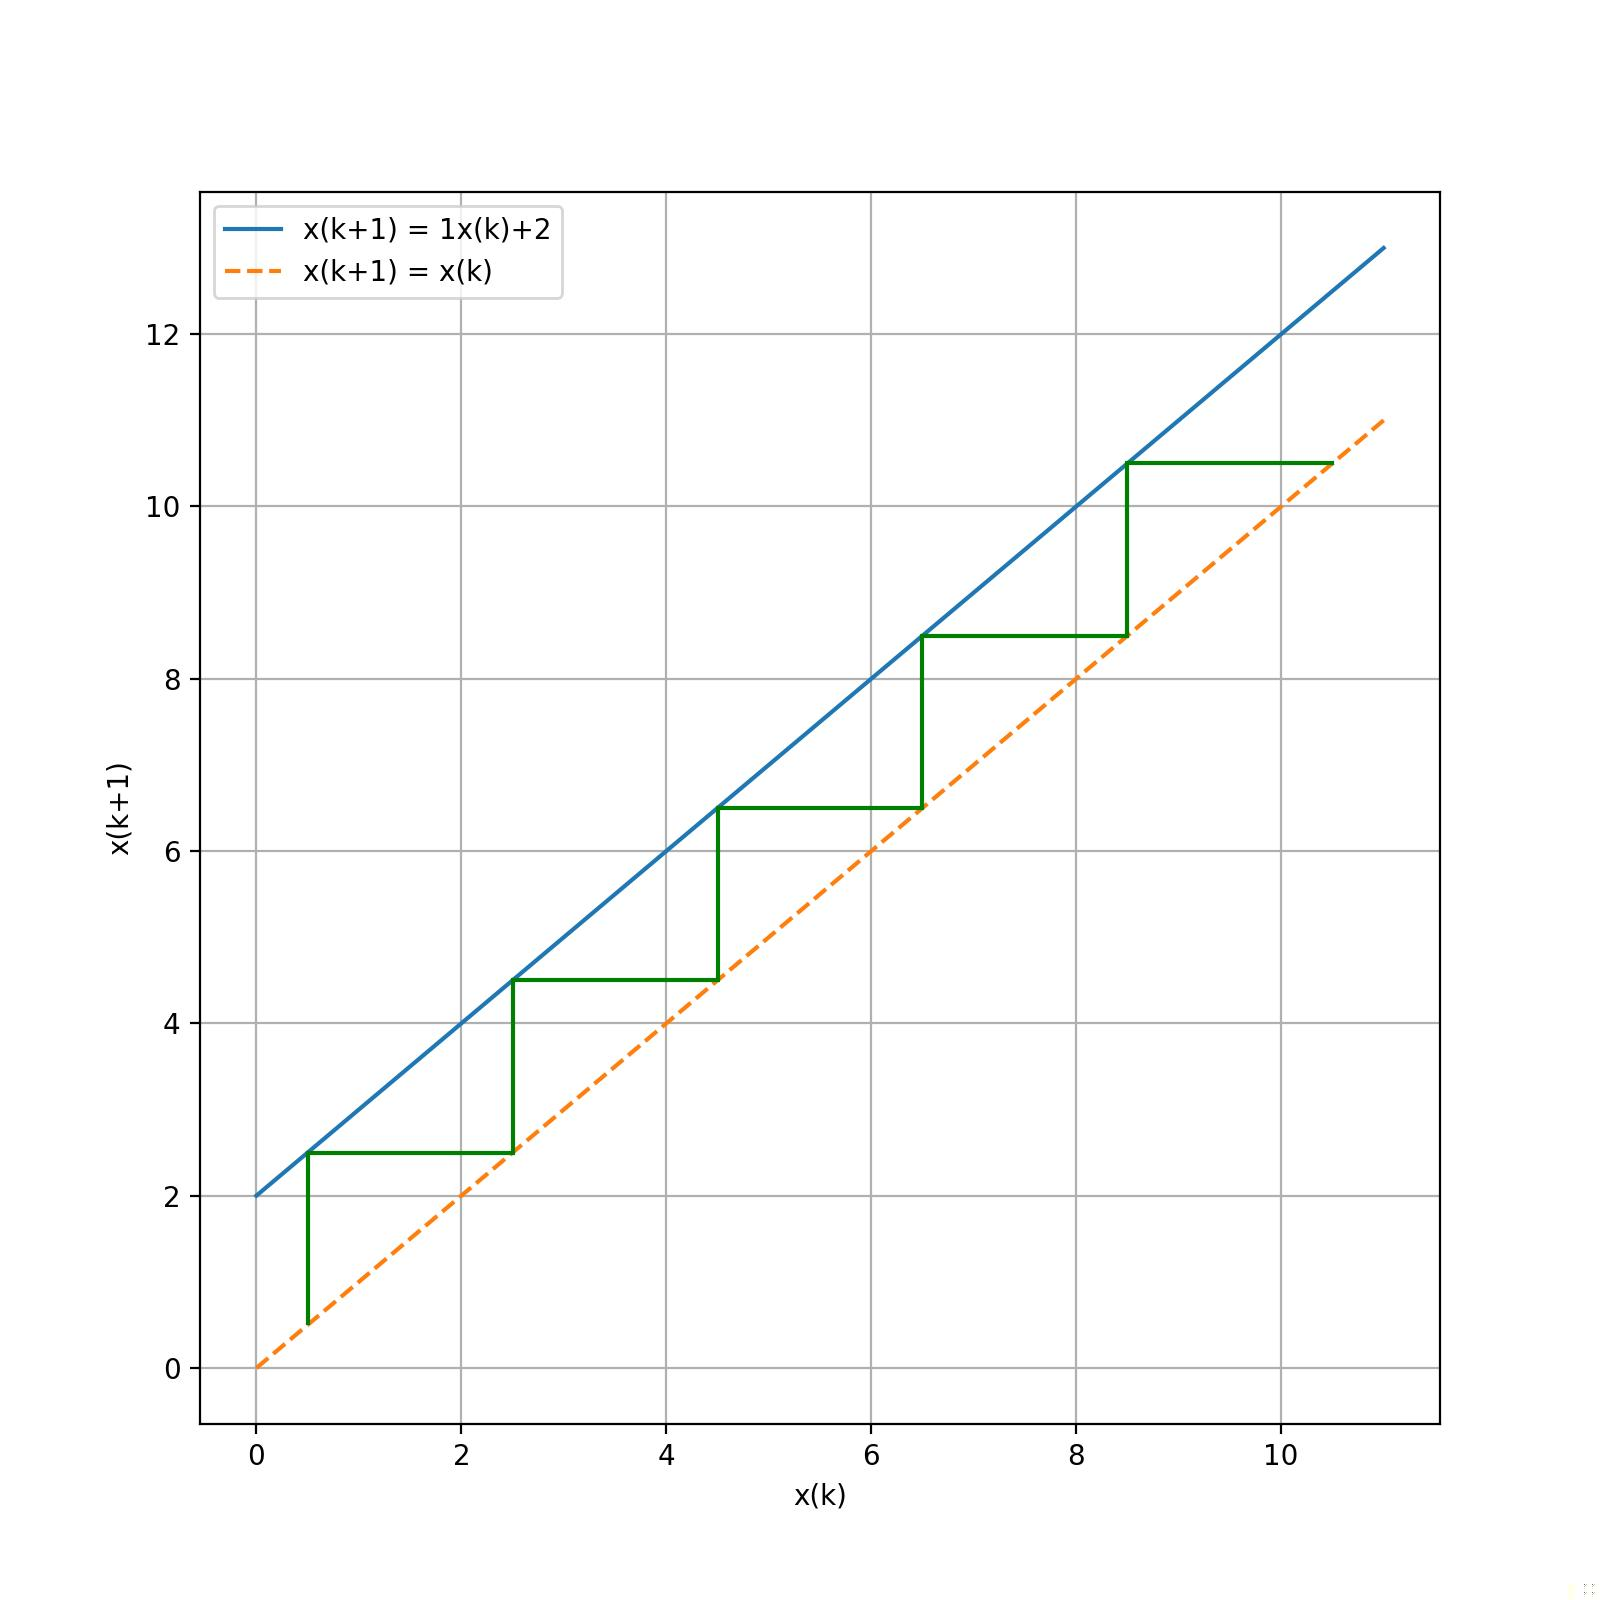
\includegraphics[width=\textwidth]{images/affine_1.jpg}
                \caption{Équation affine à un pas à trajectoire divergente}
                \label{fig:affine_1}
            \end{figure}
            Ensuite, dans la figure \ref{fig:affine_2}, on montre un cas convergent, où $a=0.75$ et $b=2$.
            \begin{figure}[ht!]
                \centering
                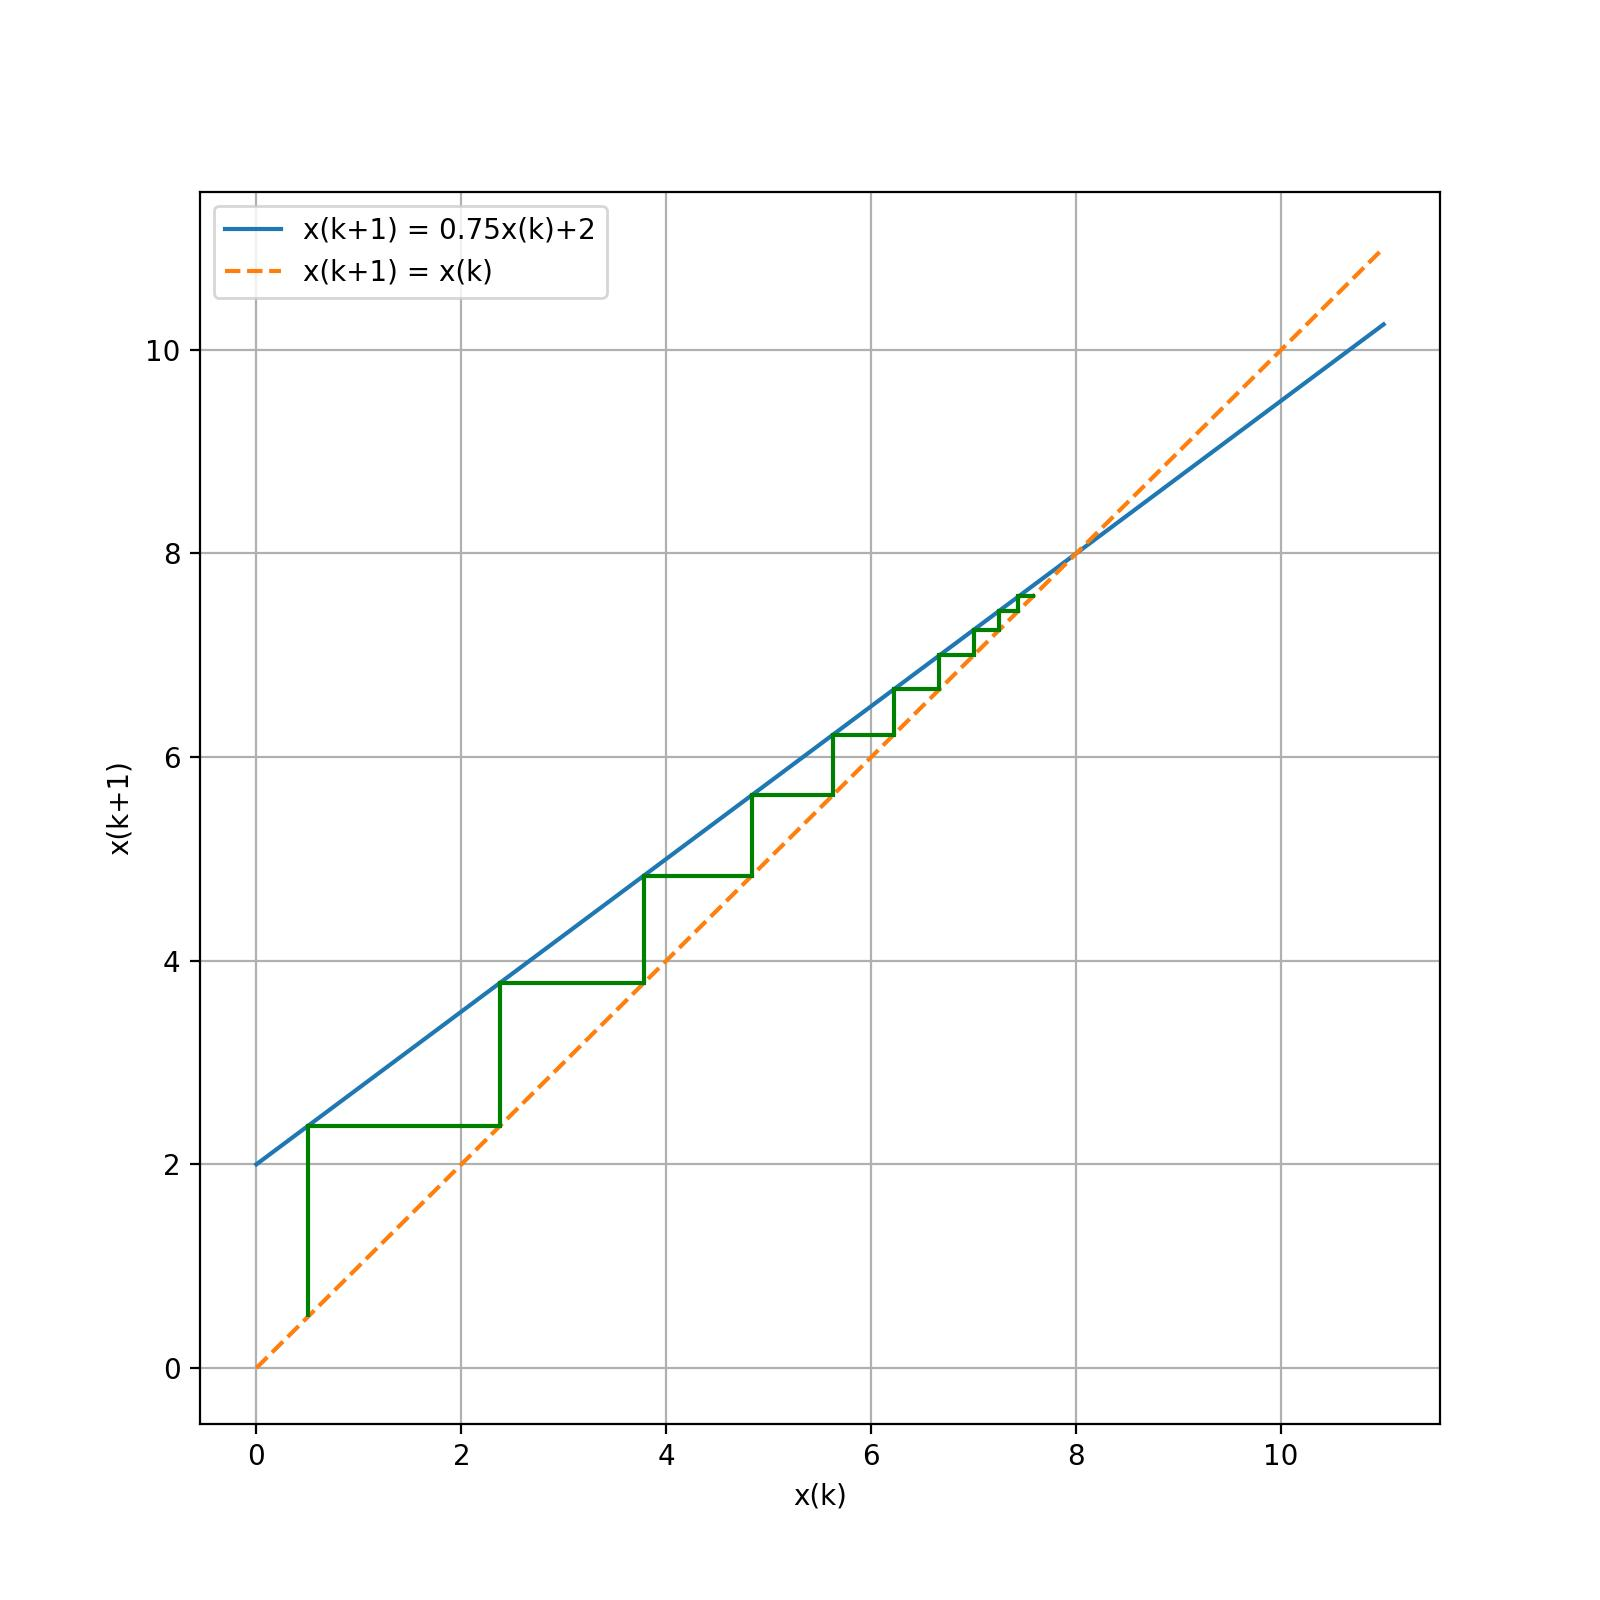
\includegraphics[width=\textwidth]{images/affine_2.jpg}
                \caption{Équation affine à un pas à trajectoire convergente}
                \label{fig:affine_2}
            \end{figure}
            Et on montre finalement dans la figure \ref{fig:affine_3} un cas oscillant, où $a=-0.5$ et $b=8$.
            \begin{figure}[ht!]
                \centering
                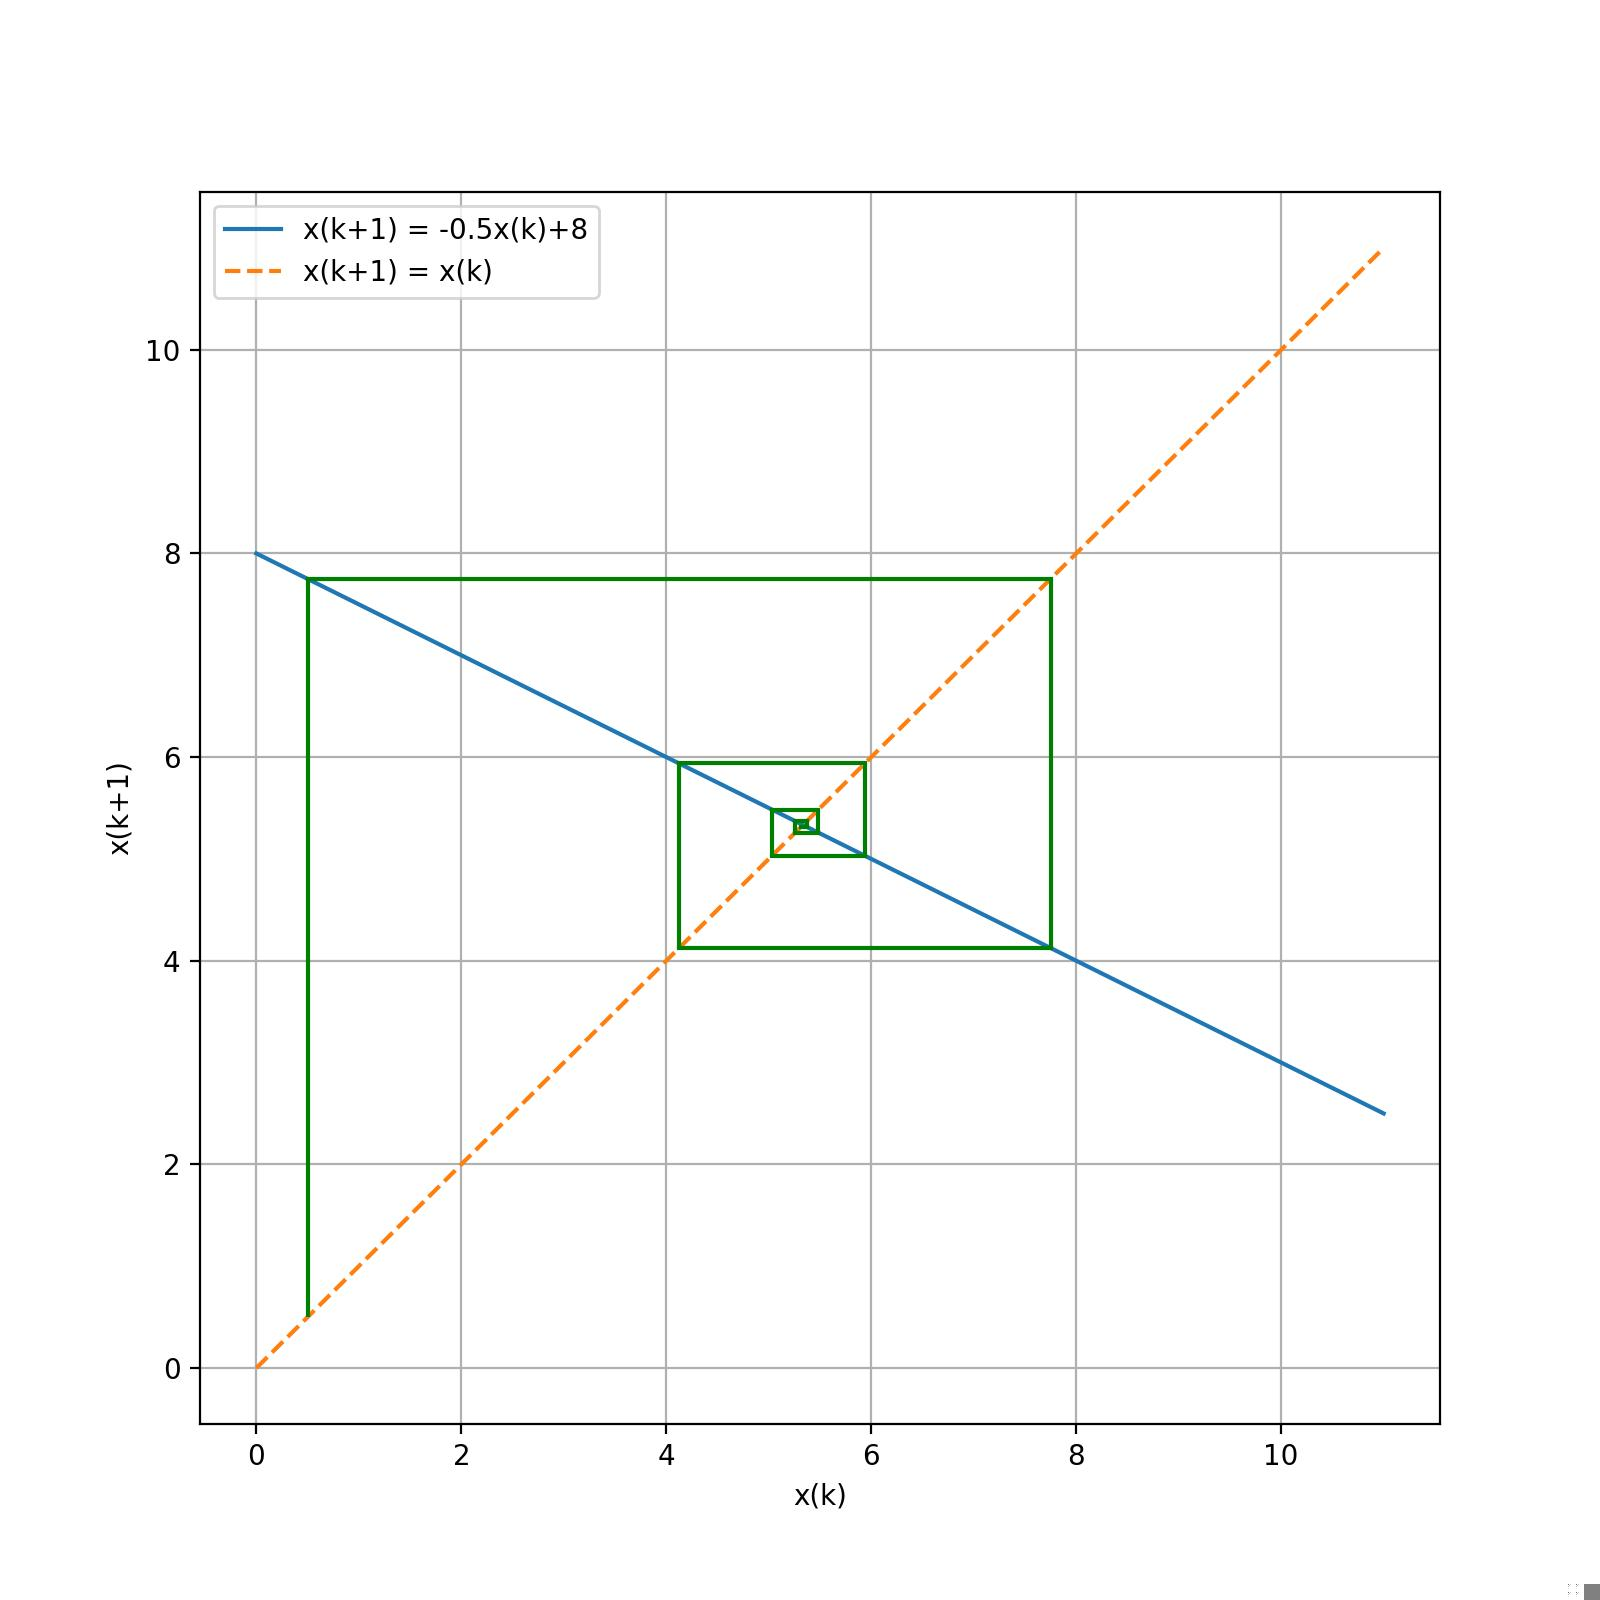
\includegraphics[width=\textwidth]{images/affine_3.jpg}
                \caption{Équation affine à un pas à trajectoire oscillante}
                \label{fig:affine_3}
            \end{figure}
            
    \section{Équations non-linéaires à un pas}
        La méthode graphique montrée précédemment illustre le principe de composition sous-jacent: la projection de la solution $x(k+1)$ sur la droite $x(k+1)=x(k)$ équivaut à reprendre la fonction $x(k+1)$ sur la valeur calculée. Analytiquement, la méthode se traduit par les étapes suivantes:
        \begin{itemize}
            \item on fixe une condition initiale $x(0)$~;
            \item on calcule la première itération: $x(1) = ax(0)+b$~;
            \item pour calculer l'itération qui suit, on utilise la valeur $x(1)$ calculée, c'est-à-dire $ax(0)+b$~;
            \item le résultat s'obtient en composant la relation avec elle-même: $x(2) = a(ax(0)+b)+b$~;
            \item le processus se répète pour les itérations qui suivent.
        \end{itemize}
        Cette méthode s'applique indépendamment de la forme de l'équation, elle peut être utilisée dans le cas non-linéaire de la même manière. Par exemple, dans la figure \ref{fig:un_pas_2}, on montre l'évolution du système décrit par l'équation $x(k+1) = \cos(x(k))$. Le code pour obtenir le graphique est donné:
        \inputminted{python}{codes/un_pas.py}
        \begin{figure}[ht!]
            \centering
            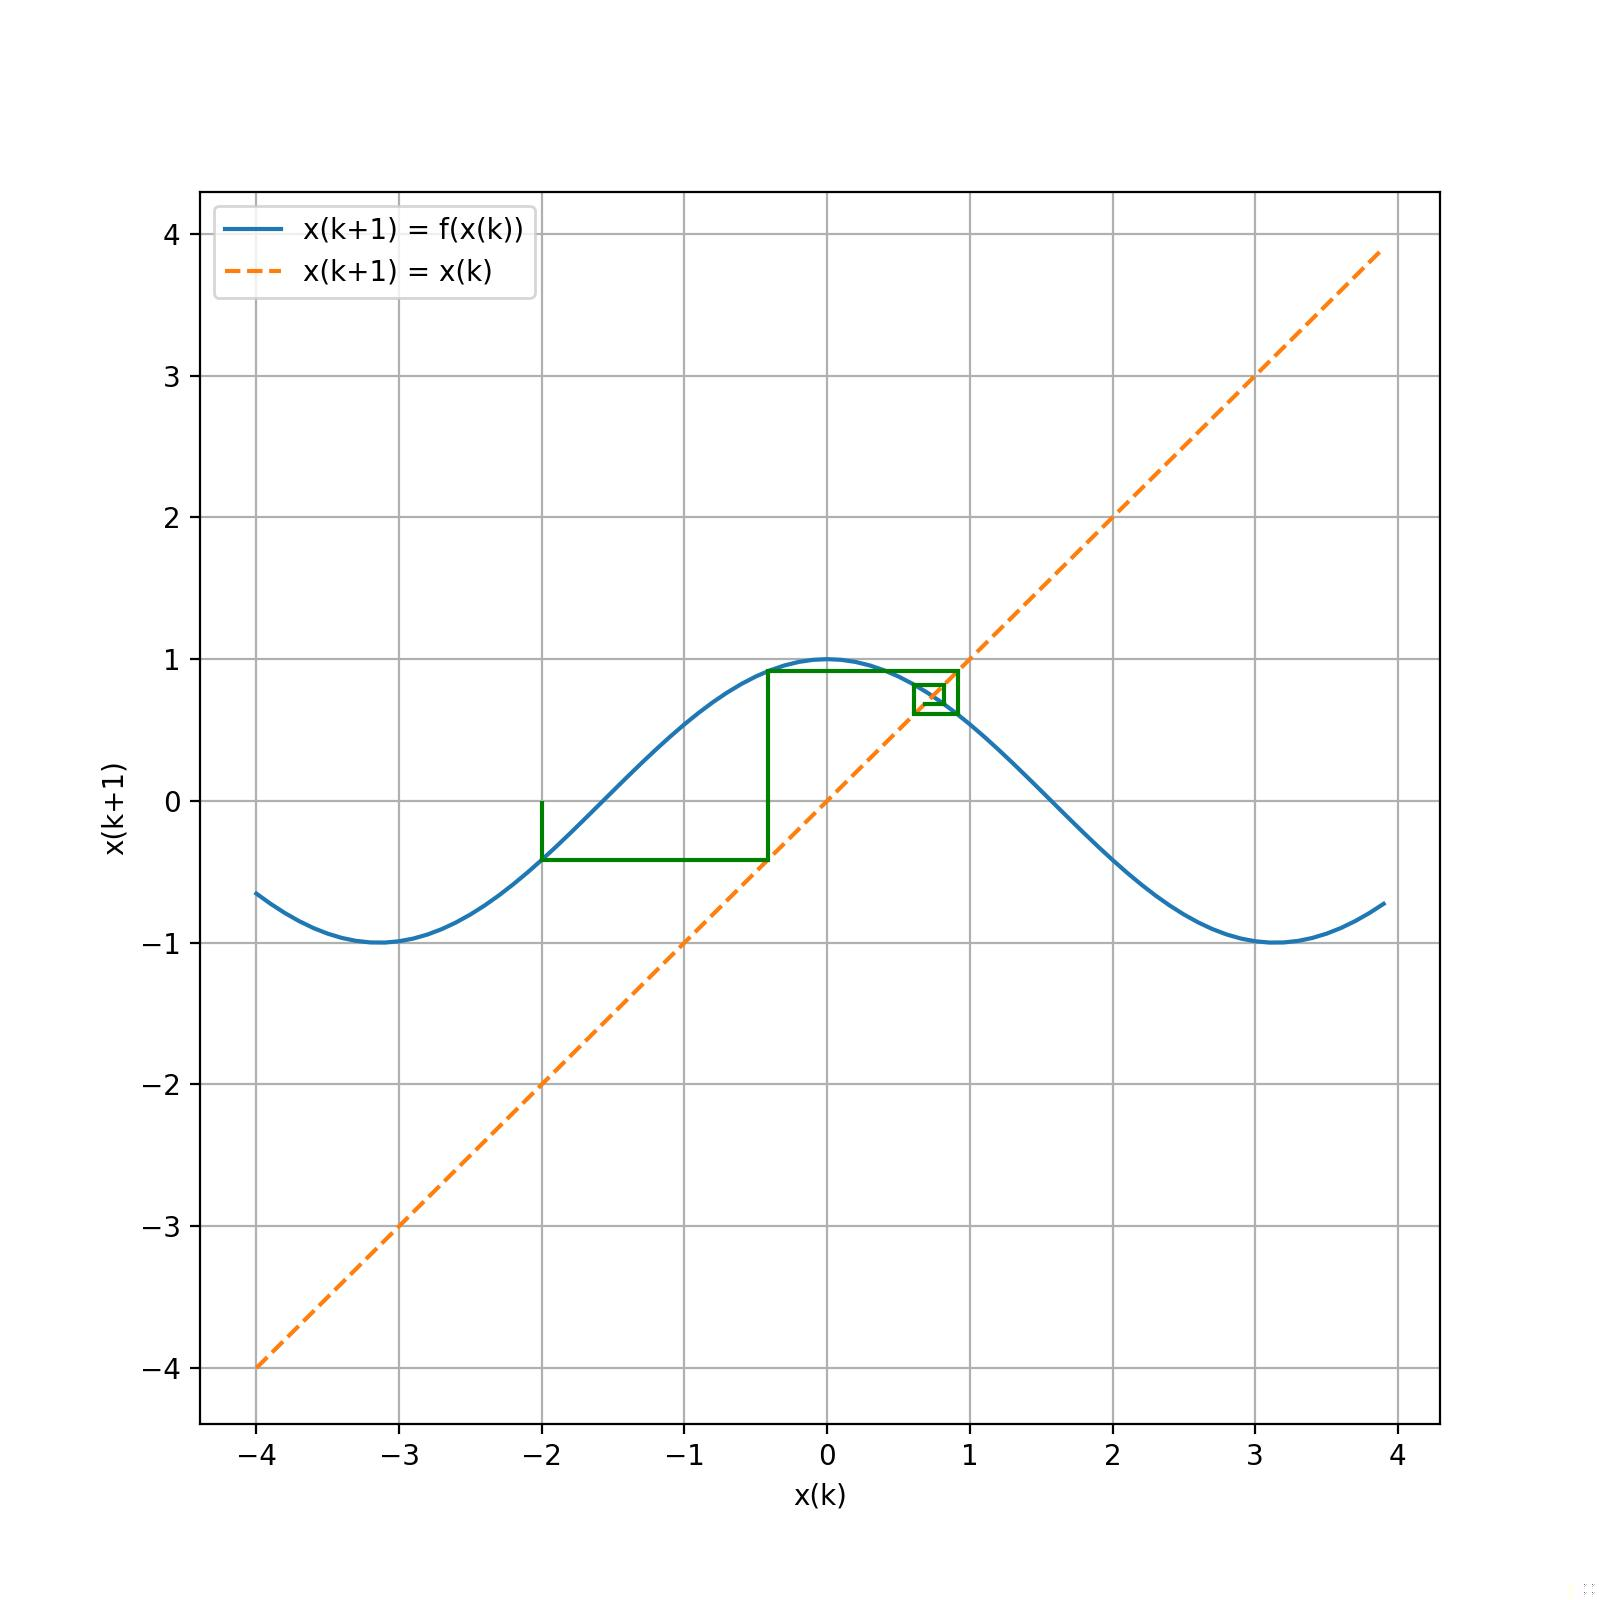
\includegraphics[width=\textwidth]{images/un_pas_2.jpg}
            \caption{Équation non-linéaire à un pas}
            \label{fig:un_pas_2}
        \end{figure}
        Cette notion de composition peut être formalisée avec la notation exponentielle: comme $x(k+1) = f(x(k))$, on peut noter 
        \begin{equation}
            \begin{split}
                x(1) = f(x(0)) \\
                x(2) = f(f(x(0))) = f^2(x(0)) \\
                \dots\\
                x(n) = f(f(\dots f(x(0)))) = f^n(x(0))
            \end{split}
        \end{equation}
        Attention à la notation. Distinguons $f^n(x)$, la \textit{$n^e$ composée de $f$}, $(f(x))^n$, la \textit{$n^e$ puissance de $f$} et $f^{(n)}(x)$, la \textit{$n^e$ dérivée de $f$}. \robin{Et évidemment on garde les notations $\cos^k$, $\sin^k$, $\log^k$, etc. pour les puissances et pas pour la composition sinon ce serait trop simple\ldots}

    \section{États d'équilibre}
        Comme dans le cas à temps continu, les points fixes ou états d'équilibre jouent un rôle important dans la description de la dynamique des systèmes.

        \begin{definition}{État d'équilibre}
            L’état $\bar{x}$ est un état d’équilibre (ou point fixe) du système $\{f, I\}$ \robin{Tu n'as pas défini la notion de \emph{système} (et à nouveau un ensemble n'est pas top, une paire ordonnée est mieux définie)} si
            \begin{equation}
                \bar{x} = f(\bar{x})
            \end{equation}
        \end{definition}
        D'un point de vue géométrique, les points d’équilibre sont les intersections sur le plan $x, y$ entre la fonction $y = f(x)$ et la droite $y = x$.
        \begin{theorem}{Existence d'un point d'équilibre}
            Soit $I = [a, b]$ un intervalle clos et borné et $f : I \to I$ une fonction continue. Alors, il existe toujours un point d’équilibre $\bar{x} \in I$ tel que $f(\bar{x}) = \bar{x}$.
        \end{theorem}

        Par exemple, le système à temps discret décrit par
        \begin{equation}
            x(k + 1) = x(k)^3
        \end{equation}
        a les points fixes $\bar{x}_1 = 0$, $\bar{x}_2 = 1$, $\bar{x}_3 = -1$. Il suffit de vérifier que la composition de la fonction par elle-même pour ces valeurs donne effectivement une valeur fixe.

    \subsection{Stabilité de l'équilibre dans les cas du premier ordre}
        \begin{definition}{Équilibre stable}
            L'équilibre est stable si pour chaque $\epsilon > 0$ il existe une constante $\delta > 0$ telle que \robin{Il manque ton quantificateur sur $k$ quelque part}
            \begin{equation}
                |x(0) - \bar{x}| < \delta \Rightarrow |x(k) - \bar{x}| < \epsilon
            \end{equation}
        \end{definition}
        \begin{definition}{Équilibre globalement asymptotiquement stable}
            L'équilibre est globalement asymptotiquement stable (ou globalement attractif) si pour chaque $x(0) \in I$
            \begin{equation}
                \lim_{k \to \infty} x(k) = \bar{x}
            \end{equation}
        \end{definition}
        \begin{definition}{Équilibre localement asymptotiquement stable}
            L'équilibre est localement asymptotiquement stable (ou localement attractif) s'il existe $\eta > 0$ telle que pour chaque $x(0) \in I \cap [\bar{x} - \eta, \bar{x} + \eta]$ 
            \begin{equation}
                \lim_{k \to \infty} x(k) = \bar{x}
            \end{equation}
        \end{definition}

        \subsection{Cycles}
            \begin{definition}{Cycle d'ordre $n$}
                Soit donné un système discret $\{f, I\}$. Un cycle d'ordre $s$ est un ensemble de $s$ valeurs différentes $\{\bar{x}_0, \dots, \bar{x}_{s-1}\}$ telles que
                \begin{equation}
                    \bar{x}_1 = f(\bar{x}_0), \quad \bar{x}_2 = f(\bar{x}_1), \dots, \quad \bar{x}_0 = f(\bar{x}_{s-1})
                \end{equation}
            \end{definition}
            La quantité $s$ est la période de l’orbite. Par exemple, le système non linéaire $\left\{ \frac{1}{x}, (0, +\infty) \right\}$ a un seul équilibre mais un nombre infini de trajectoires de période $2$.
        
            \begin{theorem}{Condition d'existence d'un cycle}
                Considérons le système discret $\{f, I\}$. La paire $\{\bar{x}_0, \bar{x}_1\}$ est un cycle d'ordre $2$ si et seulement si $\bar{x}_0$ et $\bar{x}_1$ sont des points d'équilibre de $\{f^2, I\}$ mais pas de $\{f, I\}$.
            \end{theorem}
            Par exemple, le système à temps discret
            \begin{equation}
                x(k + 1) = \frac{(2 - x(k))(3x(k) + 1)}{2}
            \end{equation}
            a un cycle d’ordre $3$ formé par les valeurs $\bar{x}_0 = 0$, $\bar{x}_1 = 1$, $\bar{x}_2 = 2$.
        \subsection{Conditions de stabilité}
        \begin{theorem}{Conditions de stabilité}
            Si $\bar{x}$ est un équilibre du système $\{f, I\}$, où $f \in C^1(I)$, alors
            \begin{itemize}
                \item $|f'(\bar{x})| < 1 \Rightarrow \bar{x}$ est localement asymptotiquement stable,
                \item $|f'(\bar{x})| > 1 \Rightarrow \bar{x}$ est instable,
                \item $|f'(\bar{x})| = 1$ ne renvoie aucune information sur la stabilité de $\bar{x}$.
            \end{itemize}
        \end{theorem}
        \begin{theorem}{Équilibre asymptotiquement stable d'une part et stable d'autre part}
            Soit $\bar{x}$ un équilibre du système $\{f, I\}$, où $f \in C^2(I)$ et $f'(\bar{x}) = 1$. Alors
            \robin{Inférieurement/supérieurement asymptotiquement (in)stable pas définis.}
            \begin{itemize}
                \item $f''(\bar{x}) > 0 \Rightarrow \bar{x}$ est inférieurement asymptotiquement stable et supérieurement instable (ou répulsif),
                \item $f''(\bar{x}) < 0 \Rightarrow \bar{x}$ est supérieurement asymptotiquement stable et inférieurement instable (ou répulsif).
            \end{itemize}
        \end{theorem}
        \begin{theorem}{Équilibre instable ou localement asymptotiquement stable}
            Soit $\bar{x}$ un équilibre du système $\{f, I\}$, où $f \in C^3(I)$, $f'(\bar{x}) = 1$ et $f''(\bar{x}) = 0$. Alors
            \begin{itemize}
                \item $f'''(\bar{x}) > 0 \Rightarrow \bar{x}$ est instable,
                \item $f'''(\bar{x}) < 0 \Rightarrow \bar{x}$ est localement asymptotiquement stable.
            \end{itemize}
            
            Soit $\bar{x}$ un équilibre du système $\{f, I\}$, où $f \in C^3$, $f(\bar{x}) = \bar{x}$ et $f'(\bar{x}) = -1$. Alors
            \begin{itemize}
                \item $2f'''(\bar{x}) + 3 (f''(\bar{x}))^2 > 0 \Rightarrow \bar{x}$ est localement asymptotiquement stable,
                \item $2f'''(\bar{x}) + 3 (f''(\bar{x}))^2 < 0 \Rightarrow \bar{x}$ est instable.
            \end{itemize}
        \end{theorem}

    \section{Exercice} 
        \begin{exercise}{Exercice}
            Trouver les cycles \robin{d'ordre 2~?} du système suivant :
            \begin{equation}
                x(k + 1) = x(k)^2 - 1
            \end{equation}
        \end{exercise}
        \begin{enumerate}
            \item Trouver les points d’équilibre du système $\{f, I\}$ :  
            Nous devons résoudre l’équation 
            \begin{equation}
                x = x^2 - 1,
            \end{equation}
            c'est-à-dire
            \begin{equation}
                x^2 - x - 1 = 0,
            \end{equation}
            dont le discriminant $\Delta$ vaut $5$, et dont les racines sont 
            \begin{equation}
                x_{1,2} = \frac{1 \pm \sqrt{5}}{2}.
            \end{equation}
            \item Trouver les points d’équilibre du système $\{f^2, I\}$, nous avons
            \begin{equation}
                f^2 = (x^2 - 1)^2 - 1 = x^4 - 2x^2 + 1 - 1 = x^4 - 2x^2.
            \end{equation}
            Nous devons donc résoudre l’équation 
            \begin{equation}
                x^4 - 2x^2 - x = 0.
            \end{equation}
            Les solutions $0$ et $-1$ sont évidentes, ce qui nous donne la factorisation
            \begin{equation}
                x(x + 1)(x^2 - x - 1) = 0.
            \end{equation}
            L’équation $x^2 - x - 1 = 0$ a déjà été résolue ci-dessus, et a pour racines 
            \begin{equation}
                \frac{1 \pm \sqrt{5}}{2}.
            \end{equation}
            Nous avons donc 
            \begin{equation}
                \bar{x}_0 = 0, \quad \bar{x}_1 = -1, \quad \bar{x}_2 = \frac{1 + \sqrt{5}}{2}, \quad \bar{x}_3 = \frac{1 - \sqrt{5}}{2}.
            \end{equation}
            Les points $\bar{x}_0 = 0$ et $\bar{x}_1 = -1$ sont donc des points d’équilibre de $f^2$ mais pas de $f$. Ils forment donc un cycle d’ordre $2$ du système $\{f, I\}$.
        \end{enumerate}
    \section{Fonction logistique discrète}
        Le système logistique est un système caractérisé par une fonction de transition paramétrique
        \begin{equation}
            x(k + 1) = f_a(x(k)) = a x(k)(1 - x(k)), \quad a \in [0, 4], \quad x \in [0, 1]
        \end{equation}
        Malgré sa simplicité, le système peut afficher des comportements qualitativement très complexes au fur et à mesure que $a$ augmente.
        Le graphique de $f_a$ est une parabole ayant pour origine le point $\left(\frac{1}{2}, \frac{a}{4}\right)$, concave et symétrique par rapport à la droite verticale $x = \frac{1}{2}$.
        Les points fixes sont obtenus en résolvant l’équation
        \begin{equation}
            a x (1 - x) = x
        \end{equation}
        Les racines sont $ \bar{x}_1 = 0 $ et le point $\bar{x}_2 = \frac{a - 1}{a}$ pour $1 < a \leq 4$.
        Notons aussi que les trajectoires ayant comme conditions initiales $x(0) = 1$ \robin{$f_a(1) = 0$. C'est $x(0)=0$} et $x(0) = \frac{1}{a}$ sont constantes pour $k \geq 1$.
        Au fur et à mesure que le paramètre $a$ augmente, le comportement qualitatif du système change fortement.
        Afin de l’analyser, il est important de tenir en considération que
        \begin{equation}
            f(x) = a x (1 - x), \quad f'(x) = a - 2 a x, \quad f''(x) = -2 a, \quad f'''(x) = 0
        \end{equation}

        \subsection{Équilibre stable: $0 \leq a < 1$}
            Si $a \in [0, 1)$, le point d'équilibre $\bar{x}_1 = 0$ est le seul équilibre. Puisque $|f'(0)| = a < 1$, il est stable. Un exemple pour $a=0.5$ est donné en Figure \ref{fig:logistique_differences_1}.
            \begin{figure}[ht!]
                \centering
                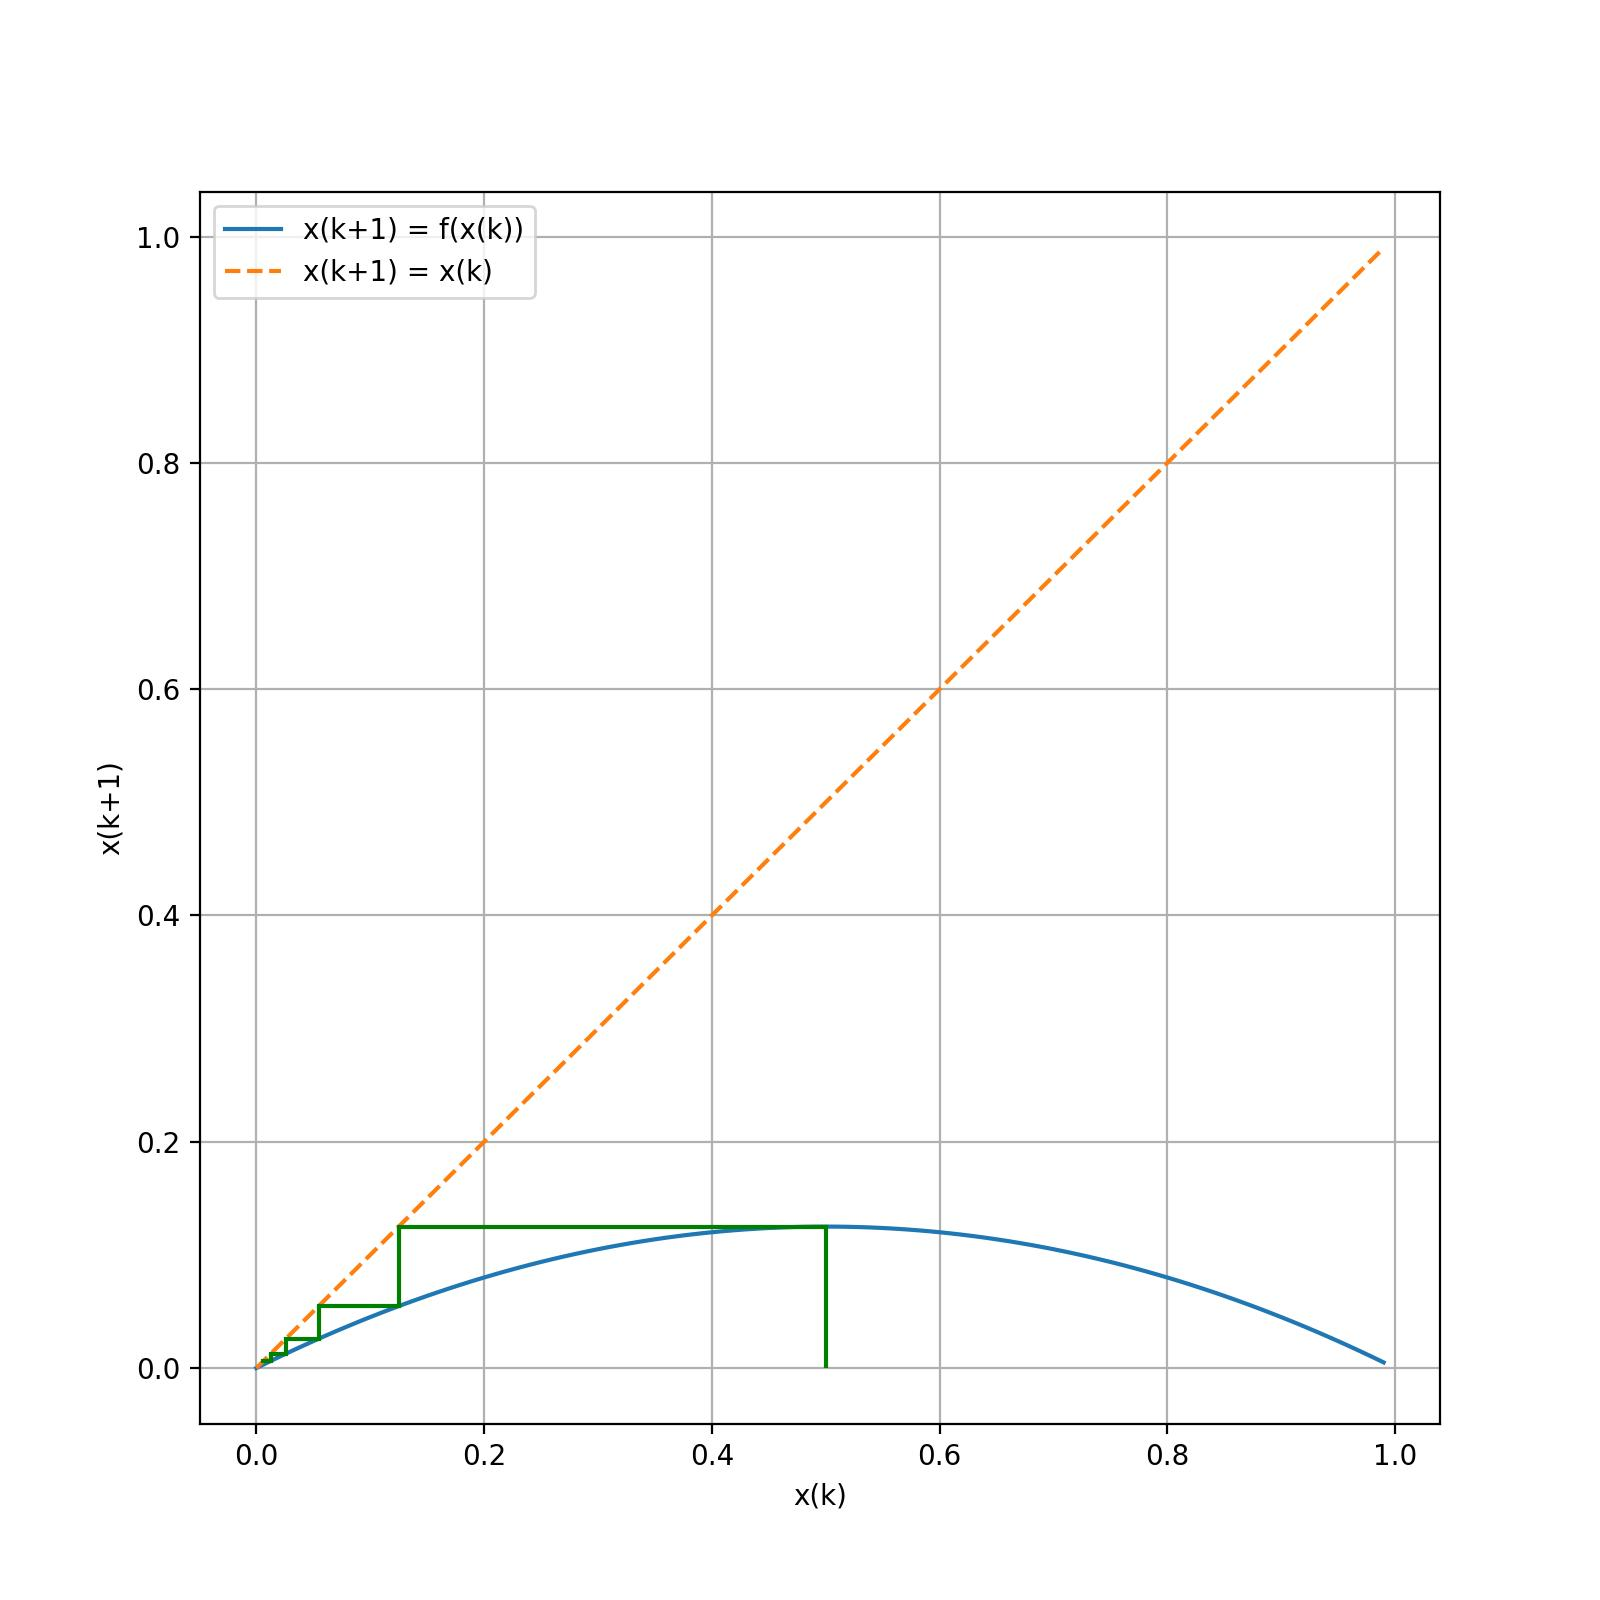
\includegraphics[width=\textwidth]{images/logistique_differences_1.jpg}
                \caption{Équation logistique pour $a=0.5$}
                \label{fig:logistique_differences_1}
            \end{figure}
            
        \subsection{Équilibre asymptotiquement stable: $a = 1$}
            Si $a = 1$, puisque $|f'(0)| = a = 1$ et $f''(0) = -2a < 0$, l'équilibre $\bar{x}_1 = 0$ est supérieurement asymptotiquement stable. Un exemple pour $a=1$ est donné en Figure \ref{fig:logistique_differences_2}.
            \begin{figure}[ht!]
                \centering
                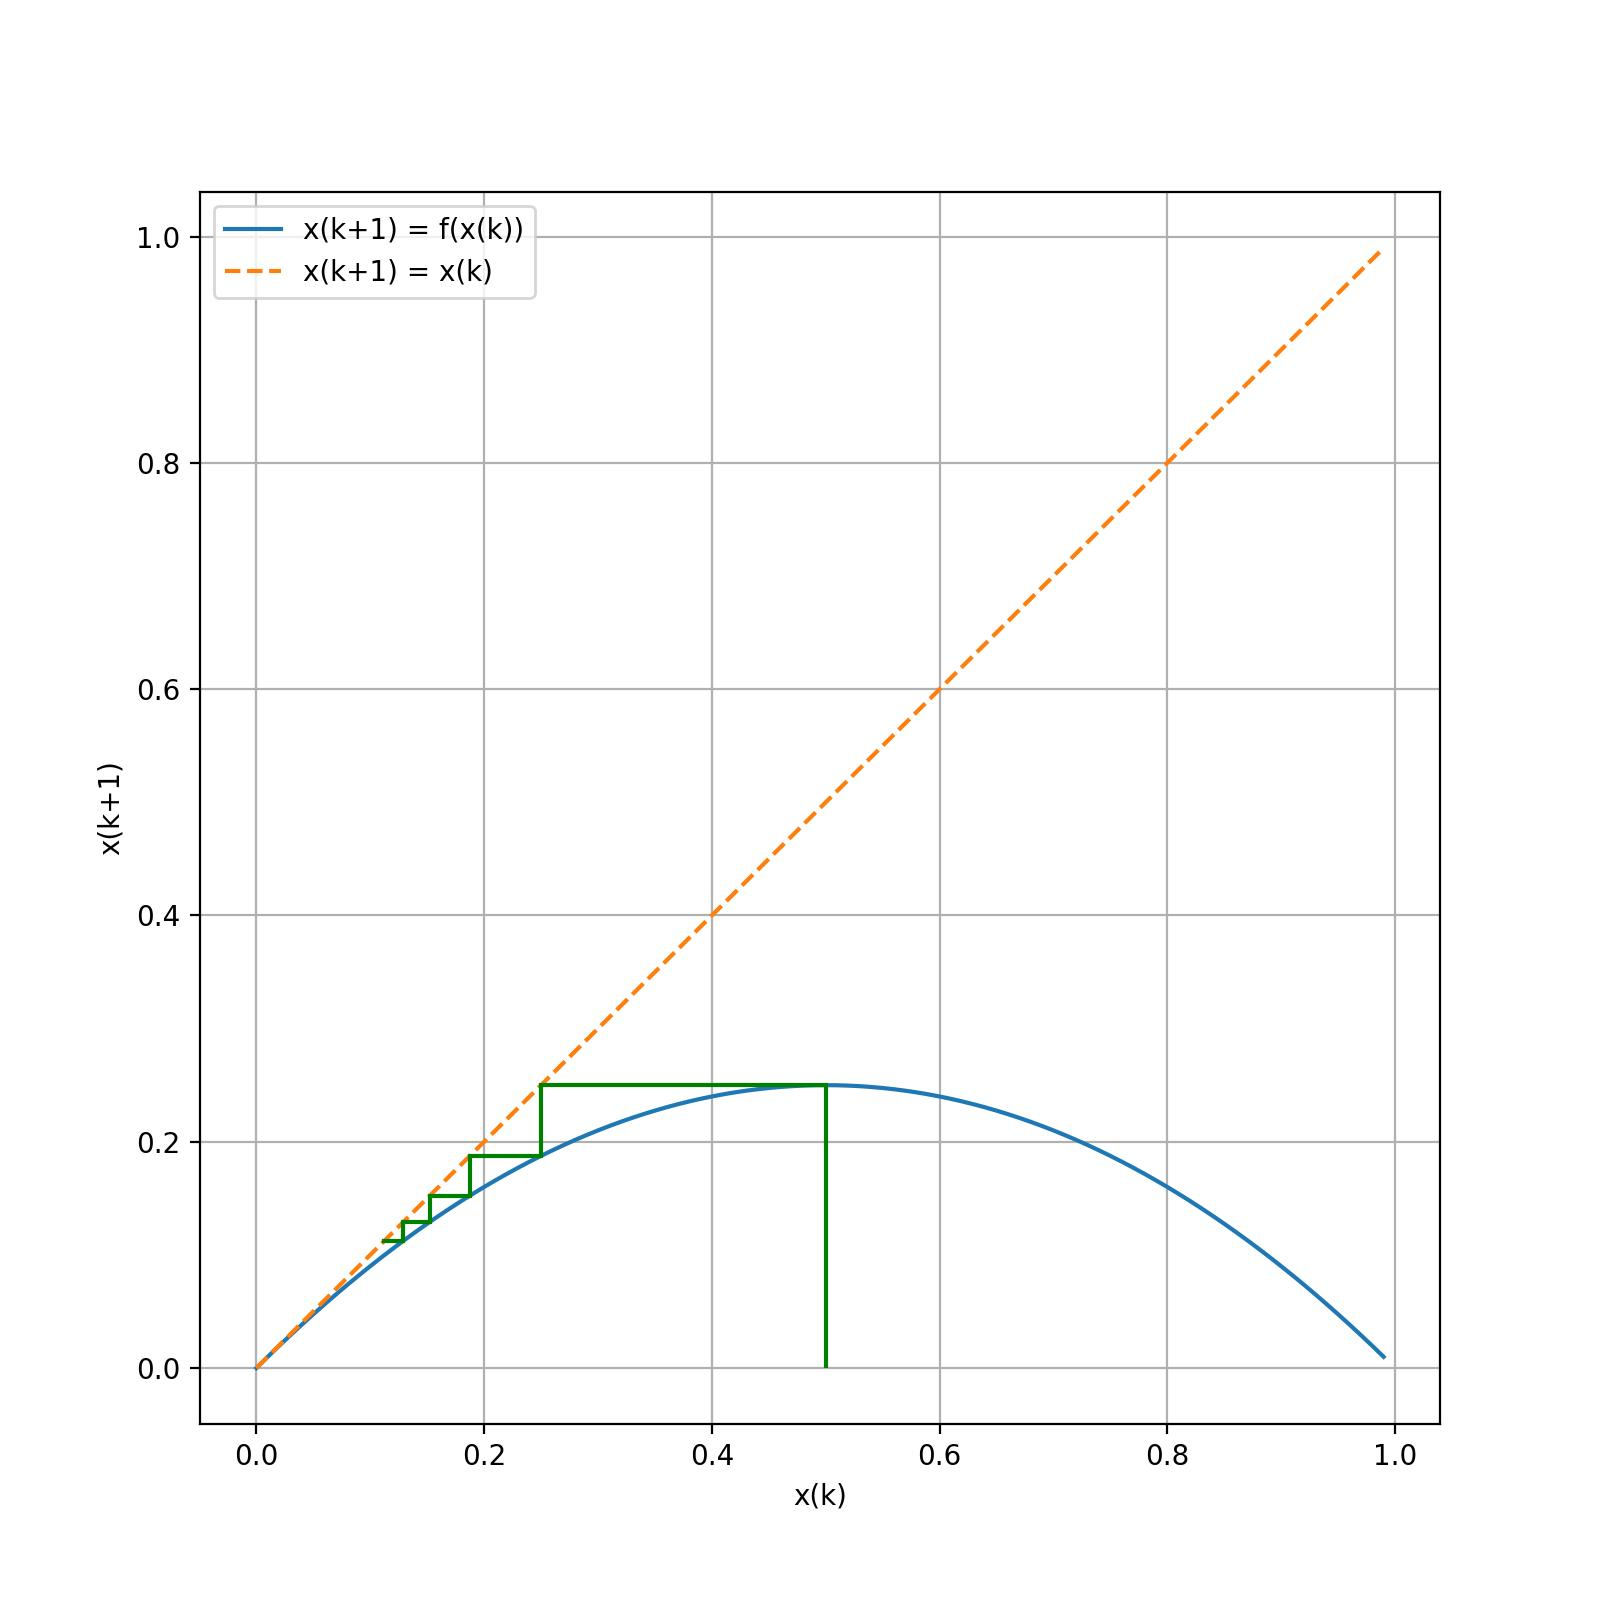
\includegraphics[width=\textwidth]{images/logistique_differences_2.jpg}
                \caption{Équation logistique pour $a=1$}
                \label{fig:logistique_differences_2}
            \end{figure}

        \subsection{Équilibre localement asymptotiquement stable, ou instable: $1 < a < 4$}
            \begin{itemize}
                \item Si $1 < a \leq 4$, nous avons deux points fixes : $\bar{x}_1 = 0$ et $\bar{x}_2 = \frac{a - 1}{a}$.
                \item Puisque $|f'(0)| = a > 1$, le point $\bar{x}_1 = 0$ est instable.
                \item Puisque $|f'(\bar{x}_2)| = |2 - a|$, l'équilibre $\bar{x}_2$ est stable pour $1 < a < 3$.
                \item Pour $a = 3$, nous avons $f'(\bar{x}_2) = -1$, $f''(\bar{x}_2) = -2a = -6$, $f'''(\bar{x}_2) = 0$. Puisque
                \begin{equation}
                    2f'''(\bar{x}_2) + 3(f''(\bar{x}_2))^2 > 0
                \end{equation}
                alors $\bar{x}_2$ est localement asymptotiquement stable.
                \item L’équilibre $\bar{x}_2$ devient instable pour $3 < a \leq 4$.
            \end{itemize}
            Deux exemples pour $a=1.5$ sont donnés en Figures \ref{fig:logistique_differences_3} et \ref{fig:logistique_differences_4}, pour $x_0=0.1$ et $x_0=0.9$.
            \begin{figure}[ht!]
                \centering
                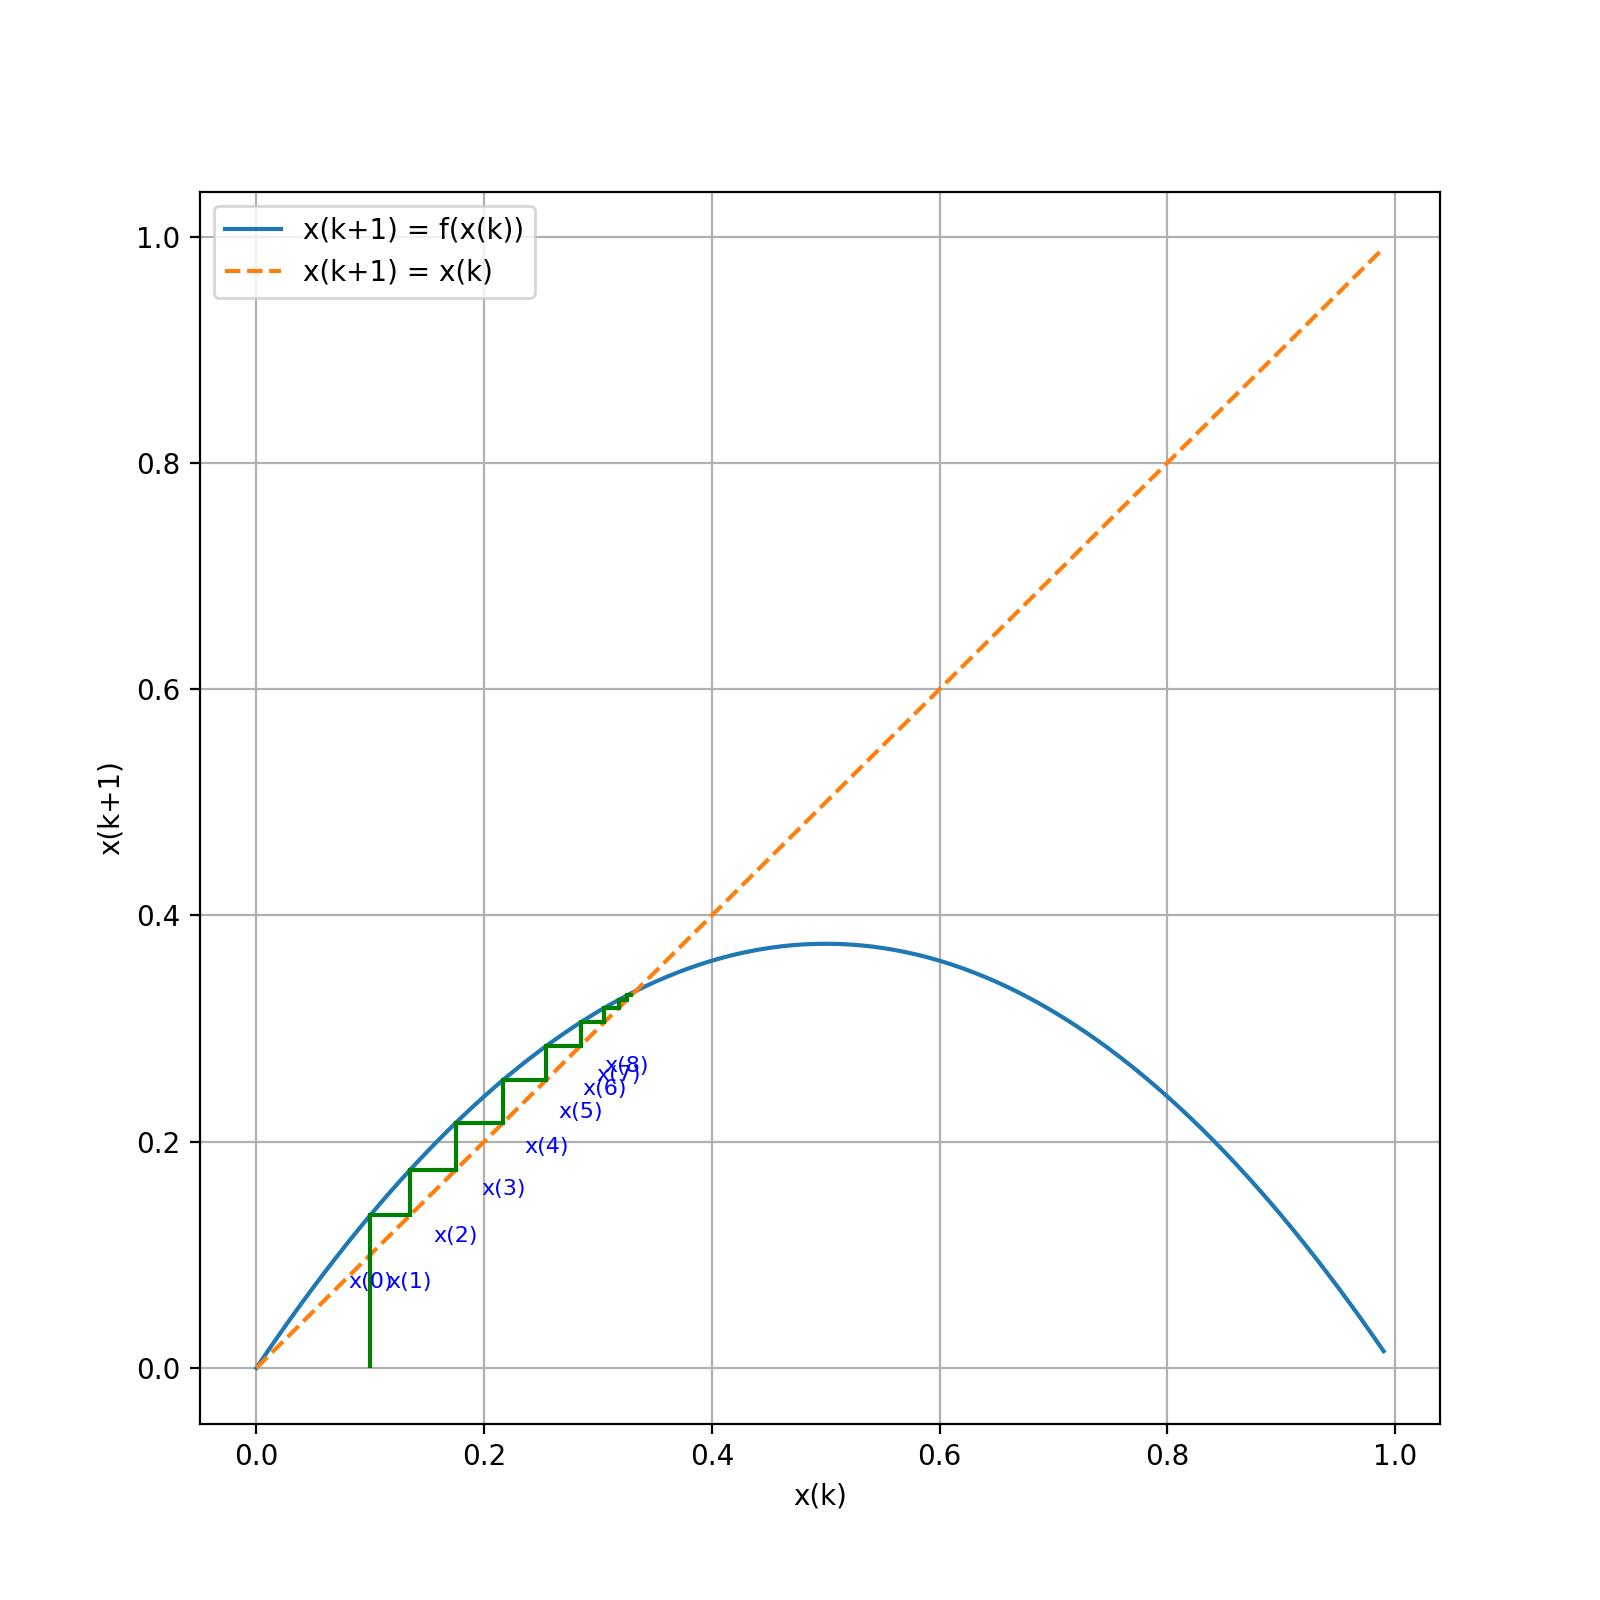
\includegraphics[width=\textwidth]{images/logistique_differences_3.jpg}
                \caption{Équation logistique pour $a=1.5$, $x_0=0.1$}
                \label{fig:logistique_differences_3}
            \end{figure}
            \begin{figure}[ht!]
                \centering
                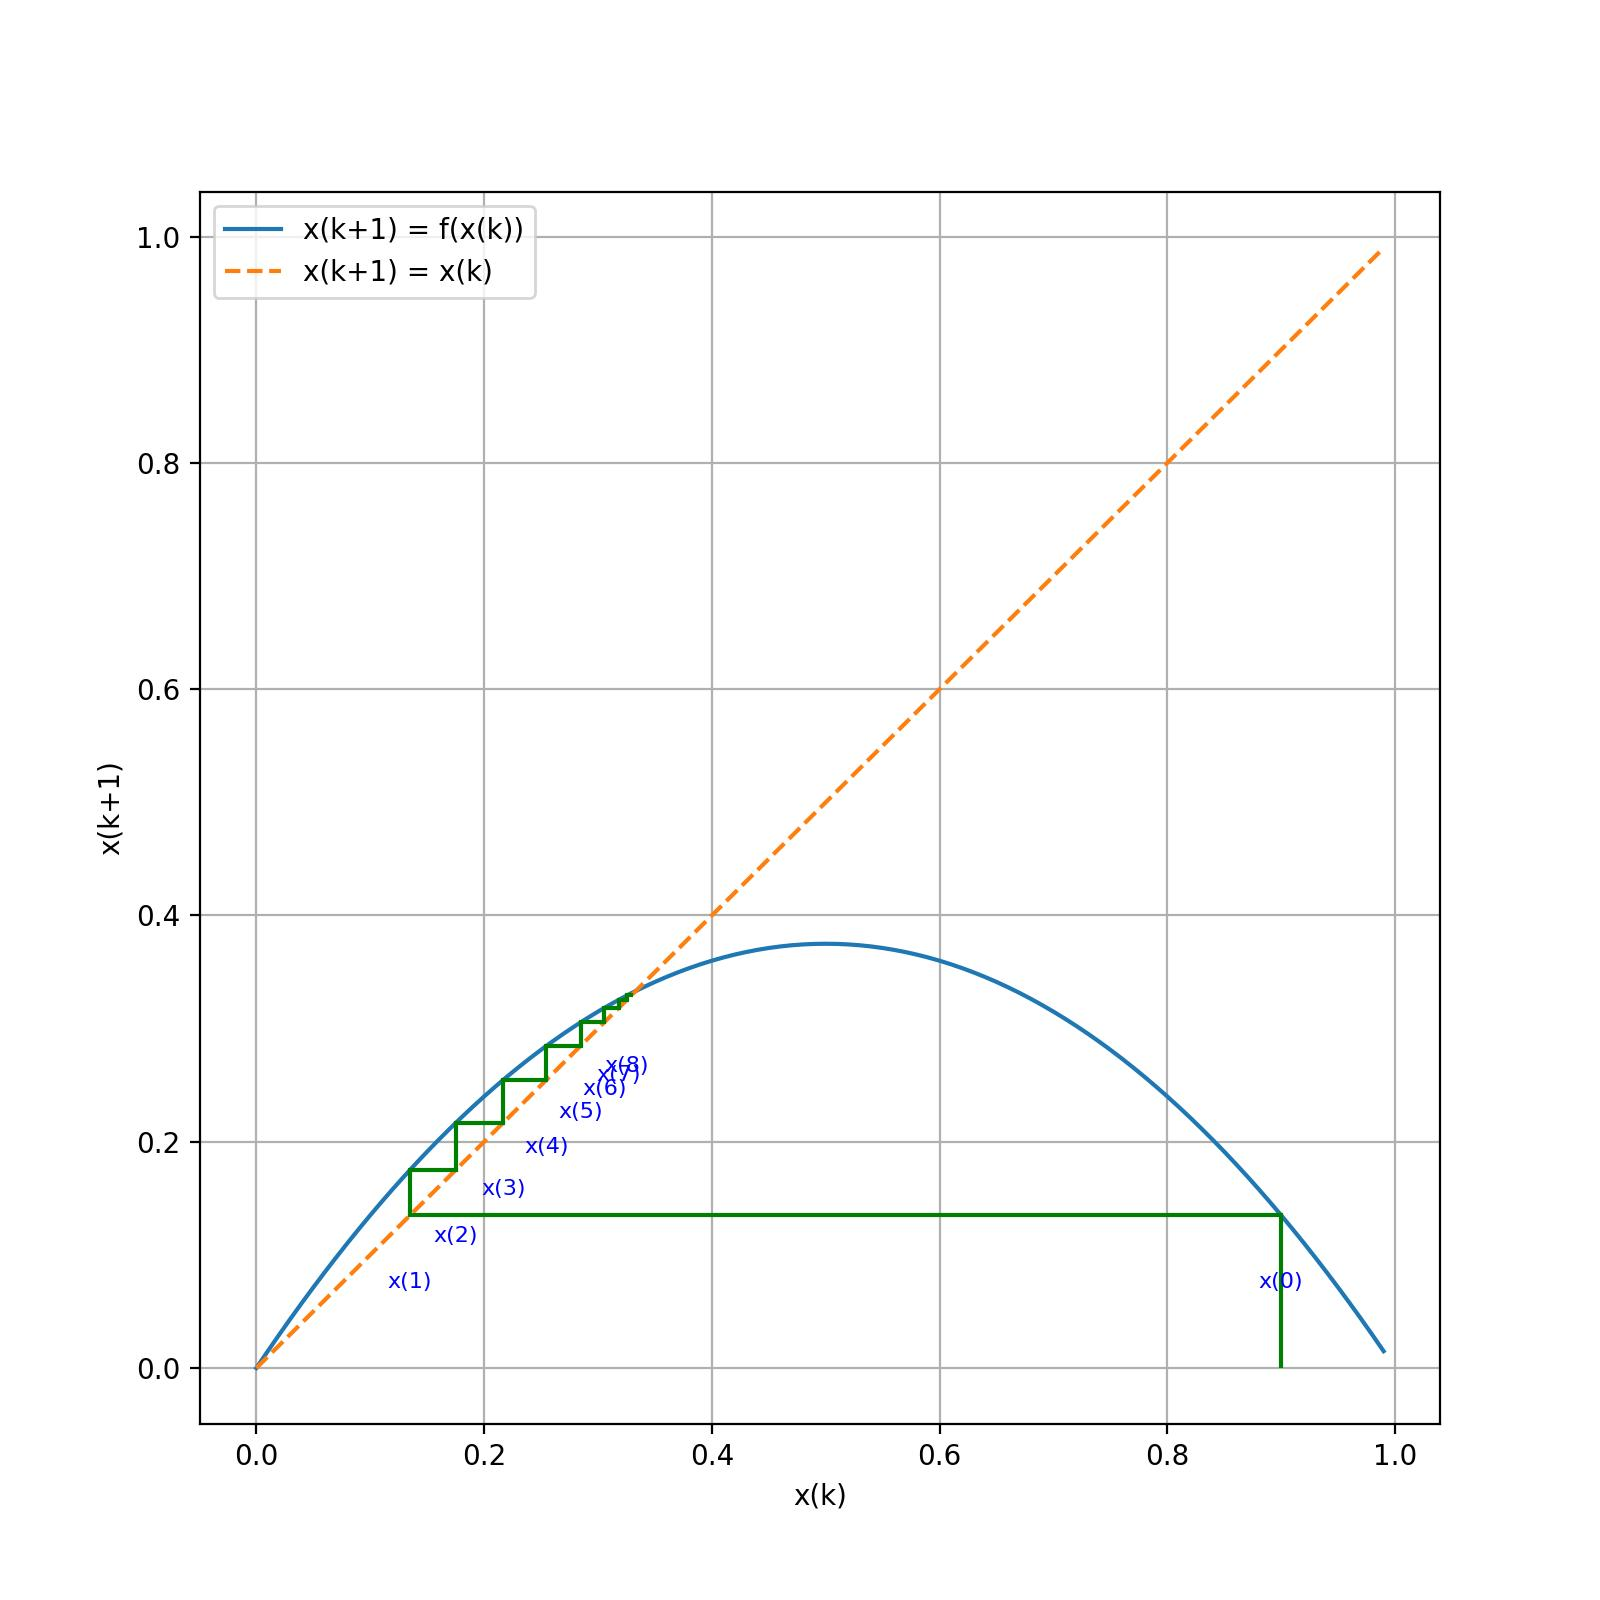
\includegraphics[width=\textwidth]{images/logistique_differences_4.jpg}
                \caption{Équation logistique pour $a=1.5$, $x_0=0.9$}
                \label{fig:logistique_differences_4}
            \end{figure}

            \subsubsection{Exemple: $a = 3$}
                L’équilibre est localement asymptotiquement stable pour $a = 3$.
                Une trajectoire est donnée en Figure \ref{fig:logistique_differences_5}.
                \begin{figure}[ht!]
                    \centering
                    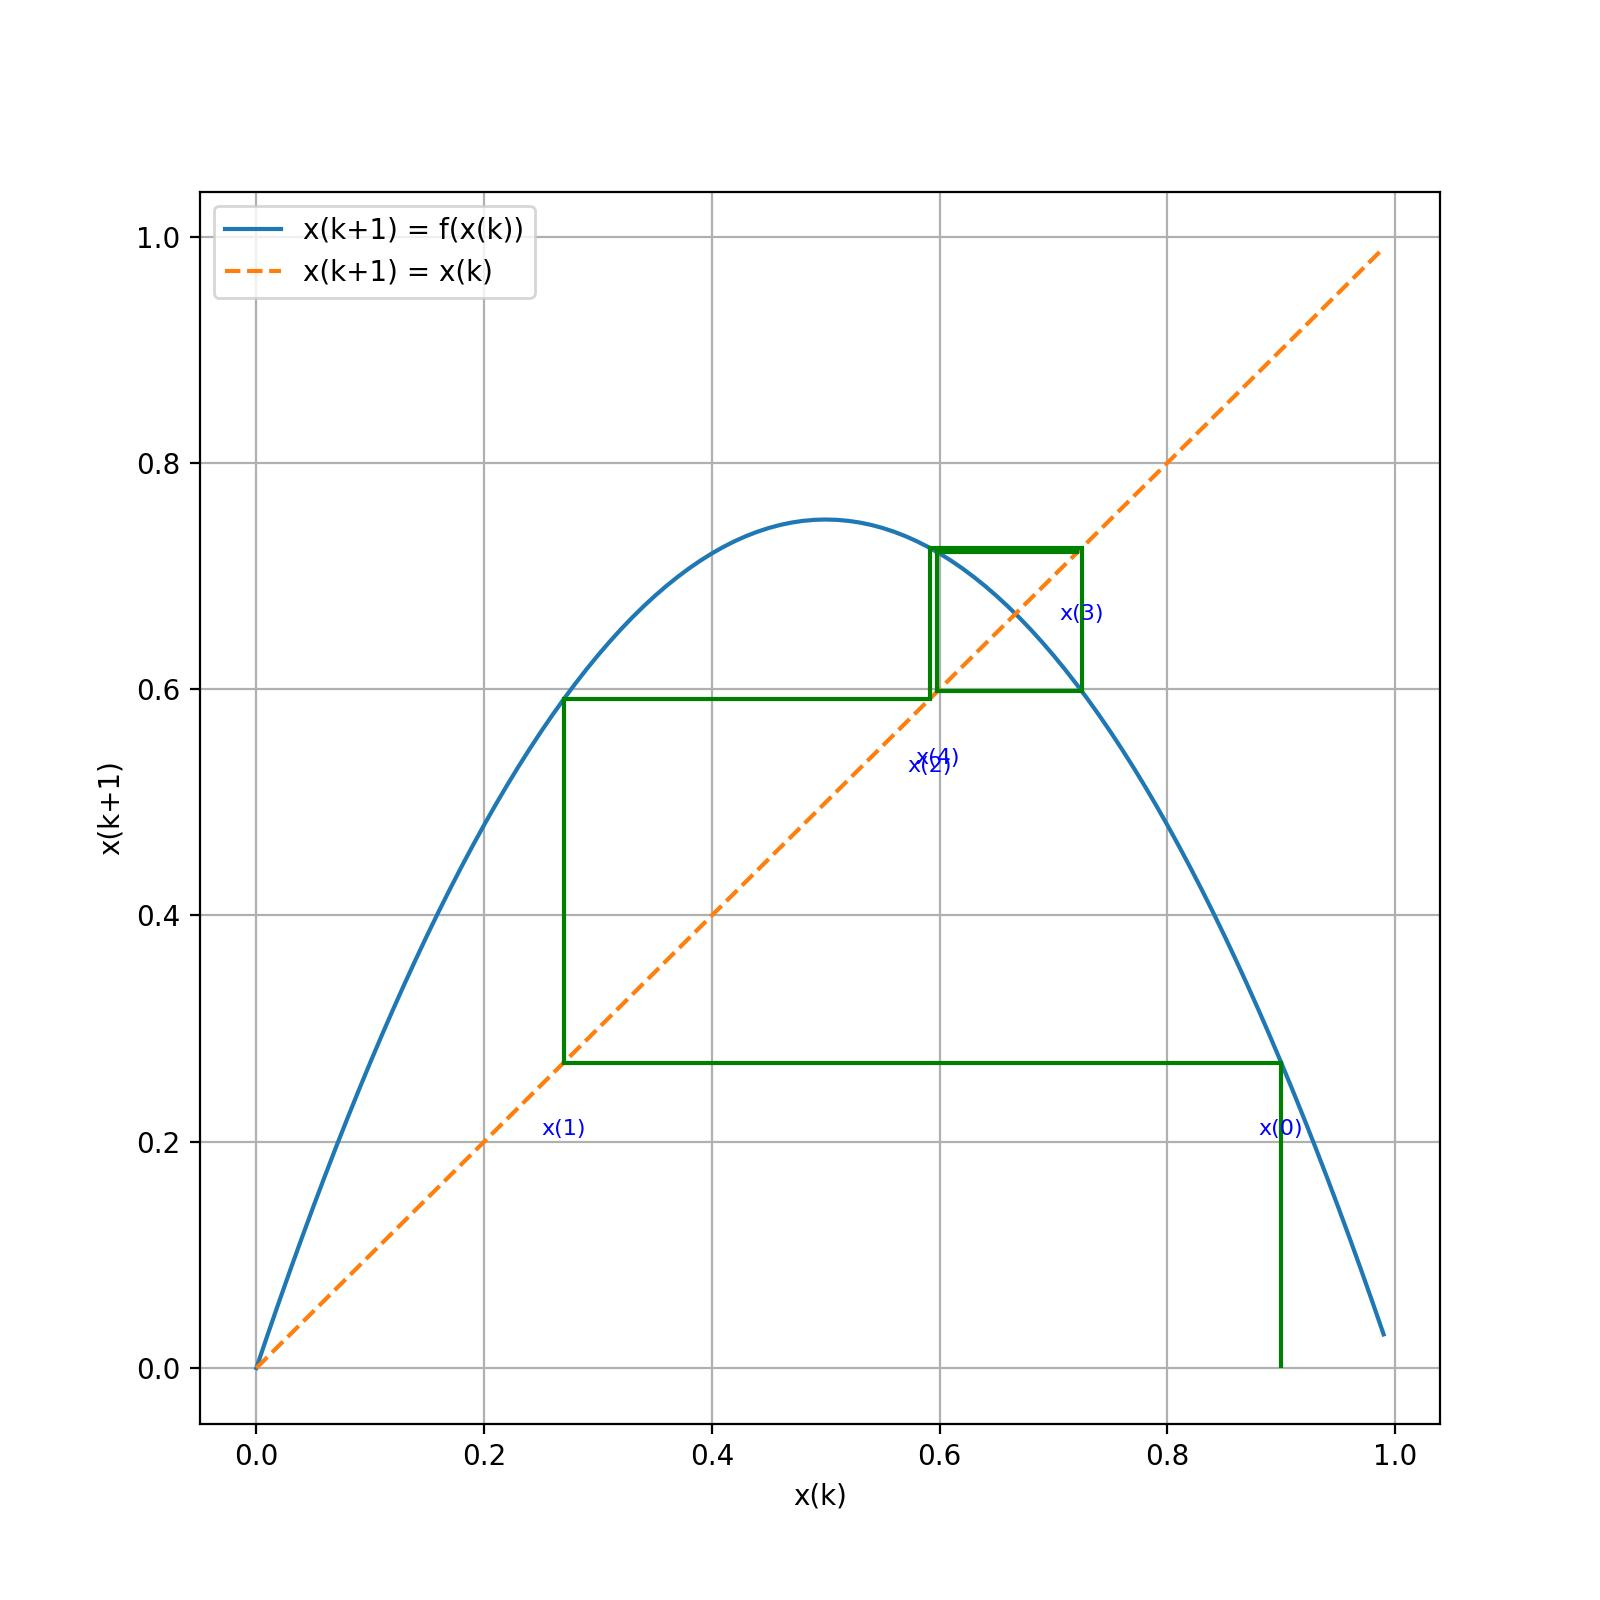
\includegraphics[width=\textwidth]{images/logistique_differences_5.jpg}
                    \caption{Équation logistique pour $a=3$}
                    \label{fig:logistique_differences_5}
                \end{figure}
            
            \subsubsection{Exemple: $a = 3.3$}
                Pour $a = 3.3 < 1 + \sqrt{6}$, l’équilibre est instable pour $3 < a < 4$.
                Un cycle stable d’ordre 2 apparaît. Une trajectoire est donnée en Figure \ref{fig:logistique_differences_6}.
                \begin{figure}[ht!]
                    \centering
                    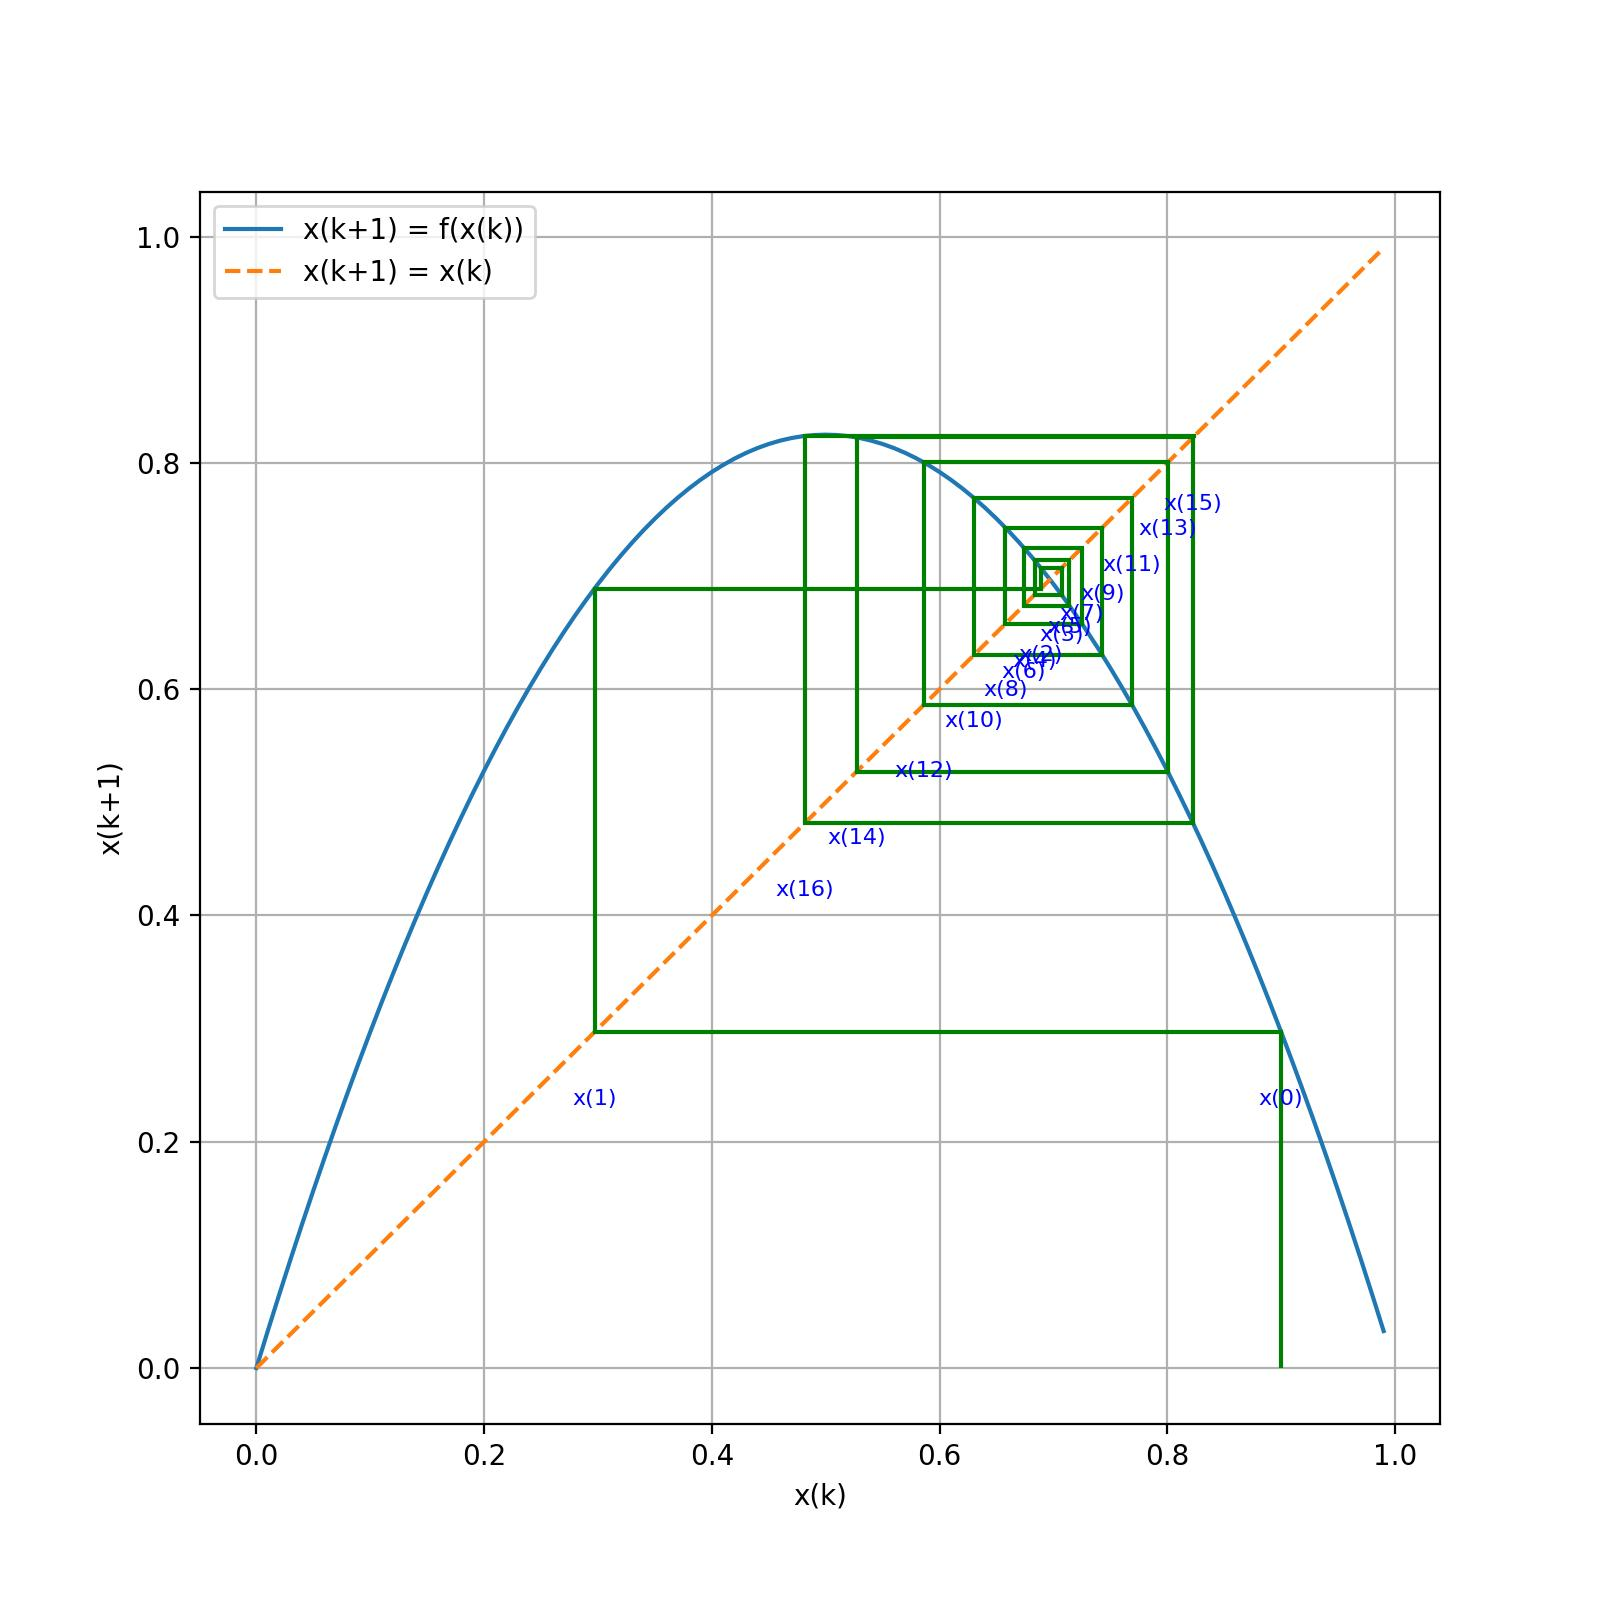
\includegraphics[width=\textwidth]{images/logistique_differences_6.jpg}
                    \caption{Équation logistique pour $a=3.3$}
                    \label{fig:logistique_differences_6}
                \end{figure}
            
                En fait, si $3 < a \leq 4$, un cycle de période $2$ apparaît. Ceci est vérifié par le fait que
                \begin{equation}
                    \begin{split}
                        &f^2(x) = a^2 x(1 - x)(1 - ax(1 - x)) = x \\
                        \Rightarrow& x = \frac{x(a - 1)}{a} \left( -a^3 x^2 + (a^2 + a^3)x - (a^2 + a) \right) = 0
                    \end{split}
                \end{equation}
                qui a quatre solutions distinctes : $\bar{x}_1$, $\bar{x}_2$ et deux solutions additionnelles
                \begin{equation}
                    \beta = \frac{a + 1 + \sqrt{(a - 3)(a + 1)}}{2a}, \quad \gamma = \frac{a + 1 - \sqrt{(a - 3)(a + 1)}}{2a}.
                \end{equation}